\documentclass[Journal,letterpaper]{ascelike-new}

% Some useful packages...
\usepackage[utf8]{inputenc}
\usepackage[T1]{fontenc}
\usepackage[round]{natbib}
\usepackage{lmodern}
\usepackage{graphicx}
\usepackage[figurename=Fig.,labelfont=bf,labelsep=period]{caption}
\usepackage{subcaption}
\usepackage{amsmath}
\usepackage{txfonts}
\usepackage{tabularx}
\usepackage[nottoc,notlot,notlof]{tocbibind} % muestra la bibliografía en TOC
\usepackage[colorlinks=true,citecolor=red,linkcolor=black]{hyperref}

\NameTag{Camus, \today}

\begin{document}


\title{Developing a MATSim Santiago Scenario: First illustrations evaluating a congestion pricing scheme}

\author[1]{Leonardo Camus}
\author[2]{Alejandro Tirachini}
\author[3]{Benjamin Kickh\"ofer}

\affil[1]{First affiliation address, with corresponding author email. Email: author.one@email.com}
\affil[2]{Second affiliation address}
\affil[2]{Third affiliation address}

\maketitle


%%%%%%%%%%%%%%%%%%%%%%%%%%%%%%%%%%%%%%%%%%%%%%%%%%%%%%%%%%%%%%%%%%%%%%%%%%%%%%%%%%%%%%%%%%%%%%%%%%%%%%%%%%%%%%%%%%%%%%%%%%%%%

% Please include an abstract:
\begin{abstract}
Summary + contributions.
\end{abstract}

\section{Introduction}

Urban agglomerations are a complex phenomenon. Taking a bottom-up perspective, cities are places where interactions occur constantly. Such a system poses different challenges in terms of both data gathering and modeling approaches, being the activity-transportation system and their interactions of particular interest. Given the constant growth of cities and the increasing concern about climate change, new methods to model and measure transport externalities properly are necessary in order to make better predictions and ultimately take better decisions.

In this work an alternative to traditional modeling approach is applied to Santiago de Chile, where each transport user is simulated as a single agent who learns from its context based on repeated iterations that represent some real conditions. This model is later compared illustratively to the classical 4-step model using a congestion pricing scenario. Since Santiago combines different transport related conditions such as pollution problems during the winter season, concentration of work and study places in the wealthier north-eastern district and the existence of a tolled urban highways network, it represents an interesting case of study for the application of a metropolitan-scale transport and activity simulator \citep{KickhoeferEtAl2016}.

The aim of this work is twofold: from one part, it represents an entry point to evaluate the general utility of this model at a metropolitan-scale in terms of both theoretical and practical terms. In addition to this, it is intended to demonstrate the capability of this approach to simulate a congestion pricing scheme and assess its impact using a classical modeling approach as a benchmark.

This paper is organized as follows: ...

%OK
\section{Literature Review: Transport system modelling approaches}
\label{sec:literature_review}
To understand transport system modeling approaches it is useful to split them into two different subsystems: demand models and assignment models, the former including everything related to people behavior and their decision processes with exception of route decisions and the latter including route choice plus all the physical models of network flows (supply models) \citep{flugel2014evaluation}. Typically, both subsystems are interacted such as demand models determine travel intensity which are subsequently used by the route-choice step, allowing the modeler to get the level of service of different network elements via the supply models. Repeating this process should finally end in an stable point which represents an equilibrium state.
%OK
Traditionally, these systems have been framed in the Four-Steps model, which in its basic version suppose the generation, distribution, modal split and assignment steps applied in a sequential manner. From its birth, research efforts have been put to a great extent into enhance the single steps of this model system \citep{Boyce2007}. In this way, generation step has evolved from growth-factor modeling to discrete choice modeling where the choice of travel frequency is used as dependent variable, distribution step has evolved from growth-factor modeling to entropy maximization models and modal split step has evolved from zonal-level models to individual choice modeling using random utility theory \citep{OrtuzarWillumsen2011}, being the logistic regression and its variants the most widely used model. Assignment, on the other hand, contains supply models, dominated by travel time-flow curves, and route choice, whose models can be classified depending on the consideration of congestion, random effects on the perception of travel costs by users, and users heterogeneity \citep{WillumsenHensherButton2008}. Drawbacks of this modeling approach can be found either in each step separately, e.g. lack of inclusion of transport costs in generation models or the fact that errors in original trip tables are replicated and amplified in forecast trip tables in the distribution step, and also when analyzing the system as a whole, usually associated with how the steps mentioned above are integrated. From a more theoretical perspective, this modeling approach has been criticized for the fact that it ignores the derived condition of travel demand from the necessity of people to engage in activities located in different points of space and time, ignoring the restrictions that emerge from the relationship between activities and trips in people's choice process \citep{McNallyAndRindt2008}.
%OK.
Examples of software that incorporate the Four Step modeling approach are Cube\footnote{http://www.citilabs.com/software/}, EMME\footnote{https://www.inrosoftware.com/en/products/emme/} and Visum\footnote{https://www.ptvgroup.com/en/welcome-to-the-ptv-group/}, all of them offering the possibility to include feedback between the different steps of the model system. In addition to the already named software, ESTRAUS offers the possibility to find the so called simultaneous equilibrium between demand and supply, such as the determined flows ensures consistent levels of service in distribution, modal split and assignment steps through the use of a hierarchical demand structure \citep{ESTRAUS}.
%OK
Together with the traditional approach, other ways to model how people travel have been explored. This is the case of the Activity-Based approach, in which tours or complete days are modeled and where transport users are part of synthetic populations to represent heterogeneity \citep{flugel2014evaluation}. As they represent demand models, the results of their application are generally transformed into Origin-Destination matrices to feed static assignment models, or are directly used in dynamic traffic assignment \citep{lin2008integration}. The general purpose of these models is to determine in which activities individuals participate during a certain period of time, the location and timing of these activities and the particular sequence of them, which in turn is translated to a particular transport behavior \citep{Ettema96}. Usually, it is assumed that individual activities are born from the household activity pattern, which are transferred to the household members through interactions and joint choice processes which are shaped by different types of restrictions \citep{McNallyAndRindt2008}.  A relevant example of this modeling approach is the work carried out by \cite{Mosh-1996}, who using the novel ideas of \cite{hagerstraand1970people} and other researches, propose a general framework useful to understand the choice process of individuals in terms of trips and the corresponding activities in which individuals engage, recognizing the existence of long-term choices usually associated with mobility behavior and life-style of households and their members, and some mid to short-term choices associated with trips and activity planning and its dynamics.
One possible classification of the models belonging to this approach can be found in \cite{Bhat2003}, who define the concept of episode as the discrete engagement of a person in a particular activity, classifying the models in
\begin{itemize}
    \item Single activity episode participation models,
    \item Activity episode pattern models:
    \begin{itemize}
        \item Activity episode scheduling models,
        \item Activity episode generation and scheduling models
    \end{itemize}
\end{itemize}
%OK
As the name suggests, single activity episode participation models focus on determining how different characteristics of the activities, the individuals and the relation between them and their household affects the participation in single activity episodes and one or more of the activity characteristics (such as duration or location). Activity episode scheduling models look for determine how individuals create sequences of episodes given a basic activity set, models that have been classified as incomplete since they rely in the activity generation in an exogenous way \citep{bowman2009historical}. Finally, activity episode generation and scheduling models focus in both how activity episodes are generated and how they are sequenced, including the two fundamental pieces that define people's choice process and which underlies the observable behaviour (as cited in \cite{Scott2002875}, pp. 877). One relevant example of this category is the model of \cite{Bowman20011} who based on the work of \cite{Mosh-1996}, present the activity generation and scheduling as a sequence of choices using a nested Logit formulation.

%A more recent overview of the activity-based modeling approach can be found in ... The general conclusion is ...%THERE ARE TWO REFERENCES THAT ARE MISSING HERE: BOYCE (2015) AND HESAM ET AL. (2018). It would be good to add them in order to close the chapter of the activity-based modelling.
%ok.

While the activity-based modelling represents an alternative demand modelling approach, dynamic traffic assignment is considered the alternative of static assignment. In general terms, dynamic assignment takes into account the fact that flows are time-varying in every link of the network, including also other characteristics such as the consideration of First-In-First-Out queue models, queue dissipation in finite time, and the existence of a capacity that is not exceeded \citep{OrtuzarWillumsen2011}. This family of models consider two general types of solution: equilibrium and not-equilibrium states \citep{friesz2007analytical}. \cite{peeta2001foundations} classify these models in two main categories, analytical and simulation-based ones, the former formulated using mathematical programming, optimal control or variational inequalities, the latter focused in representing the traffic propagation with sufficient reality. A relevant example in the simulation based models is the Cell Transmission Model \citep{daganzo1994cell}, which represents a numerical solution of the Kinematic Wave Model, in which traffic behavior is assumed to be similar to a fluid \citep{flugel2014evaluation}. The main challenges for the application of simulation-based dynamic traffic assignment models in large-scale highly-congested urban networks are related to computational efficiency, scalability and model precision, existing an important trade off between efficiency and precision \citep{wei2010critical}. Another big challenge of this models' family is calibration, which consists in finding the correct values for a set of parameters $\beta_{h}^{G}$ (where $h$ represent the temporal period and $G$ the network conditions) such as supply, demand and the interaction between them is represented with enough reality by the model \citep{balakrishna2006off}. The challenges lie in the size of $\beta_{h}^{G}$ and the relation between its element, which calls for formulating correct calibration methods, usually associated to optimization \citep{balakrishna2006off}. 
%ok
An approach that has been explored in more recent years in the transport area is the agent-based modelling, which can be defined as a computational method that allows the experimentation on objects, entities or fictitious individuals (agents) that interact in a determined environment through simulation \citep{gilbert2008agent}. A relevant characteristic of this approach is that it allows to represent the learning and adaptation process of every agent, useful for complex systems where it is not possible to know every single action and behavior of the individual entities \citep{weiss1995adaptation}. Some examples of agents' learning methods are learning by instructions, learning from examples and by practice, or learning by analogy \citep{wei2010critical}. An important example of this modelling approach in the transport field is TRANSIMS, which considers traffic micro-simulation based on cellular automata \citep{smith1995transims,nagel1996parallel}. Part of the TRANSIMS developer team continued their research efforts independently, from where MATSim (Multi-Agent Transport Simulation) \citep{IntroMATSim} was born. Agent-based models act as an interface between activity-based models and dynamic traffic assignment, keeping the identity of every agent with its activity-travel chain through the simulation, taking advantage of both approaches \citep{rieser2007agent}. As agent-based models are simulation based, they suffer from the same difficulties in terms of calibration as the pure dynamic traffic assignment models that are based on simulation. Advice to calibrate this kind of models can be found in \cite{fehler2004techniques}, mentioning that calibration techniques should recognized as a first task the inter-dependency between the different model's parameters and also make use of their modular structure, aiming to reduce the complexity and the computational time of the complete process.
%ok.
\section{MATSim}
\label{sec:matsim}
In this work, MATSim was used as the modelling framework to represent the Santiago's transport system. The complete algorithm of this model is summarized graphically in Figure \ref{fig:matsim_algorithm}. 
In this model, every agent represents a transport system user, who interacts with other agents when moving from an origin to a destination through the existing infrastructure, generally represented by the road network. A MATSim simulation is formed by a predefined number of iterations that represents the repetition of an average day. Agents' interaction allow them to evaluate their activity-travel chains (also called \emph{plans}) through a performance function which is then used to model the choice process between these alternatives.
\begin{figure}
    \centering
    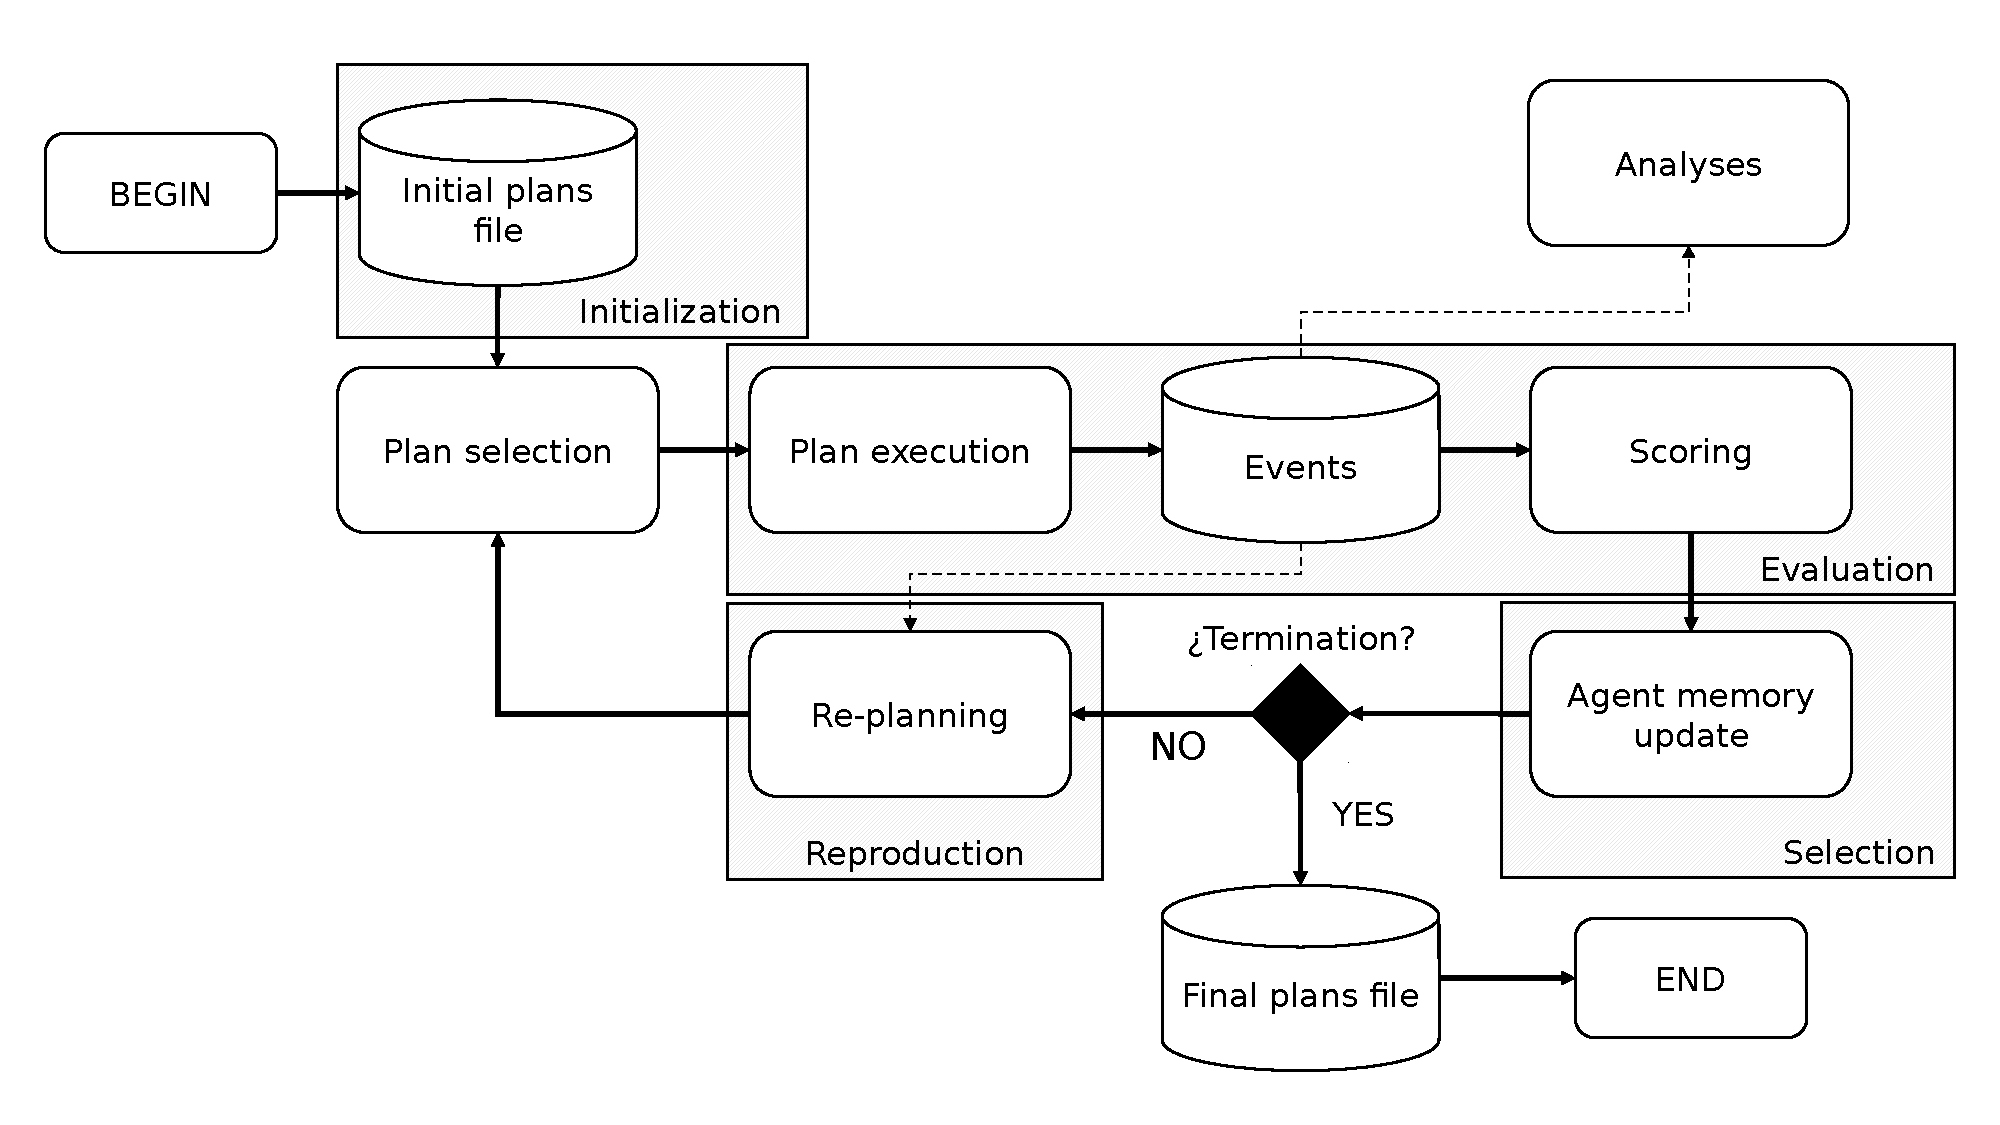
\includegraphics[scale=0.4]{images/0_algoritmo.pdf}
    \caption{MATSim algorithm. Source: \protect\cite{meister2011contribution}}
    \label{fig:matsim_algorithm}
\end{figure}
%OK.
In brief, the three steps of the algorithm are \citep{KickhoeferEtAl2016},
\begin{enumerate}
    \item Simultaneous execution of plans (mobsim): the plans of all agents are executed simultaneously on the network through the use of a first-in-first-out queue model in every link.
    \item Evaluation of plans (scoring): every agent's executed plan is evaluated with a performance function. Mathematically, the scoring function used in this work is represented by \citep{charypar2005generating} %TODO: AQUI FALTA LA UTILIDAD DE LLEGAR TARDE ETC! FOR DEPARTURE TIME CHOICE THIS IS RELEVANT!
    \begin{equation}
    S_{plan}=\sum_{q=1}^{N}(S_{act,q}+S_{trav,q})
    \end{equation}
    where $S_{act,q}$ is the utility of an activity $q$, $S_{trav,q}$ is the (typically negative) utility of travelling from activity $q$ to the next one and $N$ is the agent total number of activities. For every agent, the utility of an activity is calculated as,
    \begin{equation}
    S_{\mathit{dur,q}}=\beta_{\mathit{dur}}\cdot t_{typ,q}\cdot \ln(\mathit{t_{dur,q}}/t_{0,q})
    \end{equation}
    where $t_{typ,q}$ represents the typical duration of activity $q$, $t_{dur,q}$ is its actual duration in the simulation and $t_{0,q}$ its minimal duration. $\beta_{\mathit{dur}}$ represents the marginal utility of time as a resource. 
    The utility of traveling between two consecutive activities is computed as,
    \begin{equation}
    \label{performanceTraveling}
    S_{\mathit{trav,q}}=C_{\mathit{mode(q)}}+\beta_{\mathit{trav,mode(q)}}\cdot t_{\mathit{trav,q}}+\beta_{m}\cdot \Delta m_{q} +\beta_{m}\cdot \gamma_{\mathit{d,mode(q)}}\cdot d_{\mathit{trav,q}} + \beta_{\mathit{transfer}}\cdot x_{\mathit{transfer,q}}
    \end{equation}
    where $C_{\mathit{mode(q)}}$ is the Alternative Specific Constant (ASC), $t_{\mathit{trav,q}}$ the travel time between activity $q$ and $q+1$, $\Delta m_{q}$ the change in the monetary budget caused by fares, $\gamma_{\mathit{d,mode(q)}}$ the mode-specific monetary distance rate, $d_{\mathit{trav,q}}$ the travelled distance and $x_{\mathit{transfer,q}}$ a binary variable indicating whether a transfer occurred between the previous and the current travel leg. $\beta_{\mathit{trav,mode(q)}}$, $\beta_{m}$, $\beta_{\mathit{transfer}}$ represent the direct marginal utility of travel time, the marginal utility of income and the penalty of transfers, respectively. The specific values of the parameters used in this work are presented in Section \ref{sec:santiago_scenario}. %OK
    \item Change of plans (replanning): after executing the chosen plans, a predefined share of agents are selected to modify some aspects of a random plan already in their memory. For the Santiago scenario, it was assumed agents were able to change between car, public transport, or walk, or to explore new routes. %TODO: CHECK THIS.
\end{enumerate}
%OK
The repetition of the above steps results in an eventually stabilized scenario which is useful to further analysis.
%OK
%\begin{itemize}
%    \item Classical approaches: 4 steps model (ESTRAUS) + drawbacks: OK!
%    \item Other approaches: Activity based modelling (OK - First draft) / Agent-based models (reinforcement learning) (OK - First draft) + Dynamic Traffic Assignment (OK - First draft)
%    \item MATSim as an alternative/complement to the classical approaches. Importance of this type of modelling in the local context + drawbacks. (OK - First Draft)
%    \item Externalities: congestion pricing, but there are others.
%\end{itemize}
\newpage
\section{The MATSim Santiago Scenario}
\label{sec:santiago_scenario}
A MATSim scenario consists in all the necessary inputs used to simulate the transport system of a particular area of study. In practice, these inputs are the initial demand represented by the agents' initial plans, the network and the parameters of the behavioural models described in Section \ref{sec:matsim}, in addition to other optional elements. One of the main steps in this work was the improvement of these elements with the aim to increase the realism of the simulation.
%OK.

\subsection{Inputs Improvements}
\subsubsection{Initial plans}
The agents initial plans came from the most recent Santiago's Origin Destination Household Survey (ODS) \citep{EOD2012}, which covered 45 municipalities within the Santiago's metropolitan region. This survey was applied during the months of July 2012 to November 2013, and considered two different types of days; the \emph{normal-period days} which are the working days from the first fortnight of March to the first fortnight of December, and the \emph{summer-period or weekend days} which are all the other days not considered in the first classification \citep{munoz2016encuesta}. The final sample size of the Santiago's ODS was $18.000$ households, which were split into $11.000$ households surveyed during \emph{normal-period days} and 7000 households surveyed during \emph{summer-period or weekend days}. Expansion and correction factors were calculated and applied to the survey in order to reproduce the total number of households and persons in the study area and to represent household size and number of vehicles distributions \citep{Contreras2015}. 
%OK.
The improvements made in this work started by correcting the original initial plans determined by \cite{KickhoeferEtAl2016}, filtering out the \emph{summer-period or weekend days} which were contained on them, ending up with a population with $28.740$ agents. Naming $\pi_{0}$ the corrected initial plans, the next step was to clone every agent $i \in \pi_{0}$ a number of times proportional to its corresponding expansion factor in order to build a synthetic population representative of the 10\% of the Santiago's population. In other words, if $F_{i}$ represent the corresponding survey expansion factor, then every agent was cloned $f_{i}$ times, where
\begin{equation}
    f_{\mathit{i}}= [\eta\cdot F_{\mathit{i}}]
\end{equation}

being $\eta$ determined by,

\begin{equation}
    \eta=\frac{10\%\cdot T}{\sum\limits_{\mathit{i}\in \pi_{0}}F_\mathit{i}}
\end{equation}
%OK
The above procedure ended up in a 10\% population, $\pi_{10}^{0}$, with $665.201$ agents. Since all the clones of a particular agent contained exactly the same information as the original one, some randomization were necessary to add variability to the simulations. First, trip start times (equivalently activity end times) were randomized using Santiago's public transport smartcard data (see e.g. \cite{munizaga2012estimation}). In this case, data for the period between September 23rd and 27th of 2013 was used as the ground truth to start the randomization process. For every public transport trip of every agent in $\pi_{10}^{0}$, a new trip start time was chosen assuming it follows a normal distribution centered in the reported trip start time and a standard deviation (in minutes), $\sigma \in \{1,2,...,60\}$, to be determined based on a distance measure between the histogram built with the smartcard data times, \textbf{A}, and the public transport trip start times once already randomized, \textbf{F}, choosing $\sigma$ such as the distance between \textbf{A} and \textbf{F} was minimum. Since histograms depend on the bin size, five different sizes were used to find $\sigma$, starting in five minutes and ending with thirty minutes. Finally, for every $\sigma$ tested and for every bin size, the randomization was repeated ten times in order to get an average of the distance measure. The distance measure chosen in this case was the $\chi^2$ distance \citep{pele2010quadratic}, given by
\begin{equation}
    \chi^2(A,F)=\frac{1}{2}\sum_{\mathit{i}}^{n}\frac{(a_{\mathit{i}}-f_{\mathit{i}})^2}{(a_{\mathit{i}}+f_{\mathit{i}})}
\end{equation}

where $a_{i}$ and $f_{i}$ represent the relative frequency in each bin $i$ and $n$ the total number of bins. The above procedure ended up in a $\sigma_{\chi^2}^{*}=33$ minutes, which was found to be the parameter that minimizes the distance between \textbf{A} and \textbf{F} (see Figure \ref{histogram_comparition}). 
Finally, this parameter was used for all the trips of the whole cloned population, ending up with a population $\pi_{10}^{1}$.

\begin{figure}
    \centering
    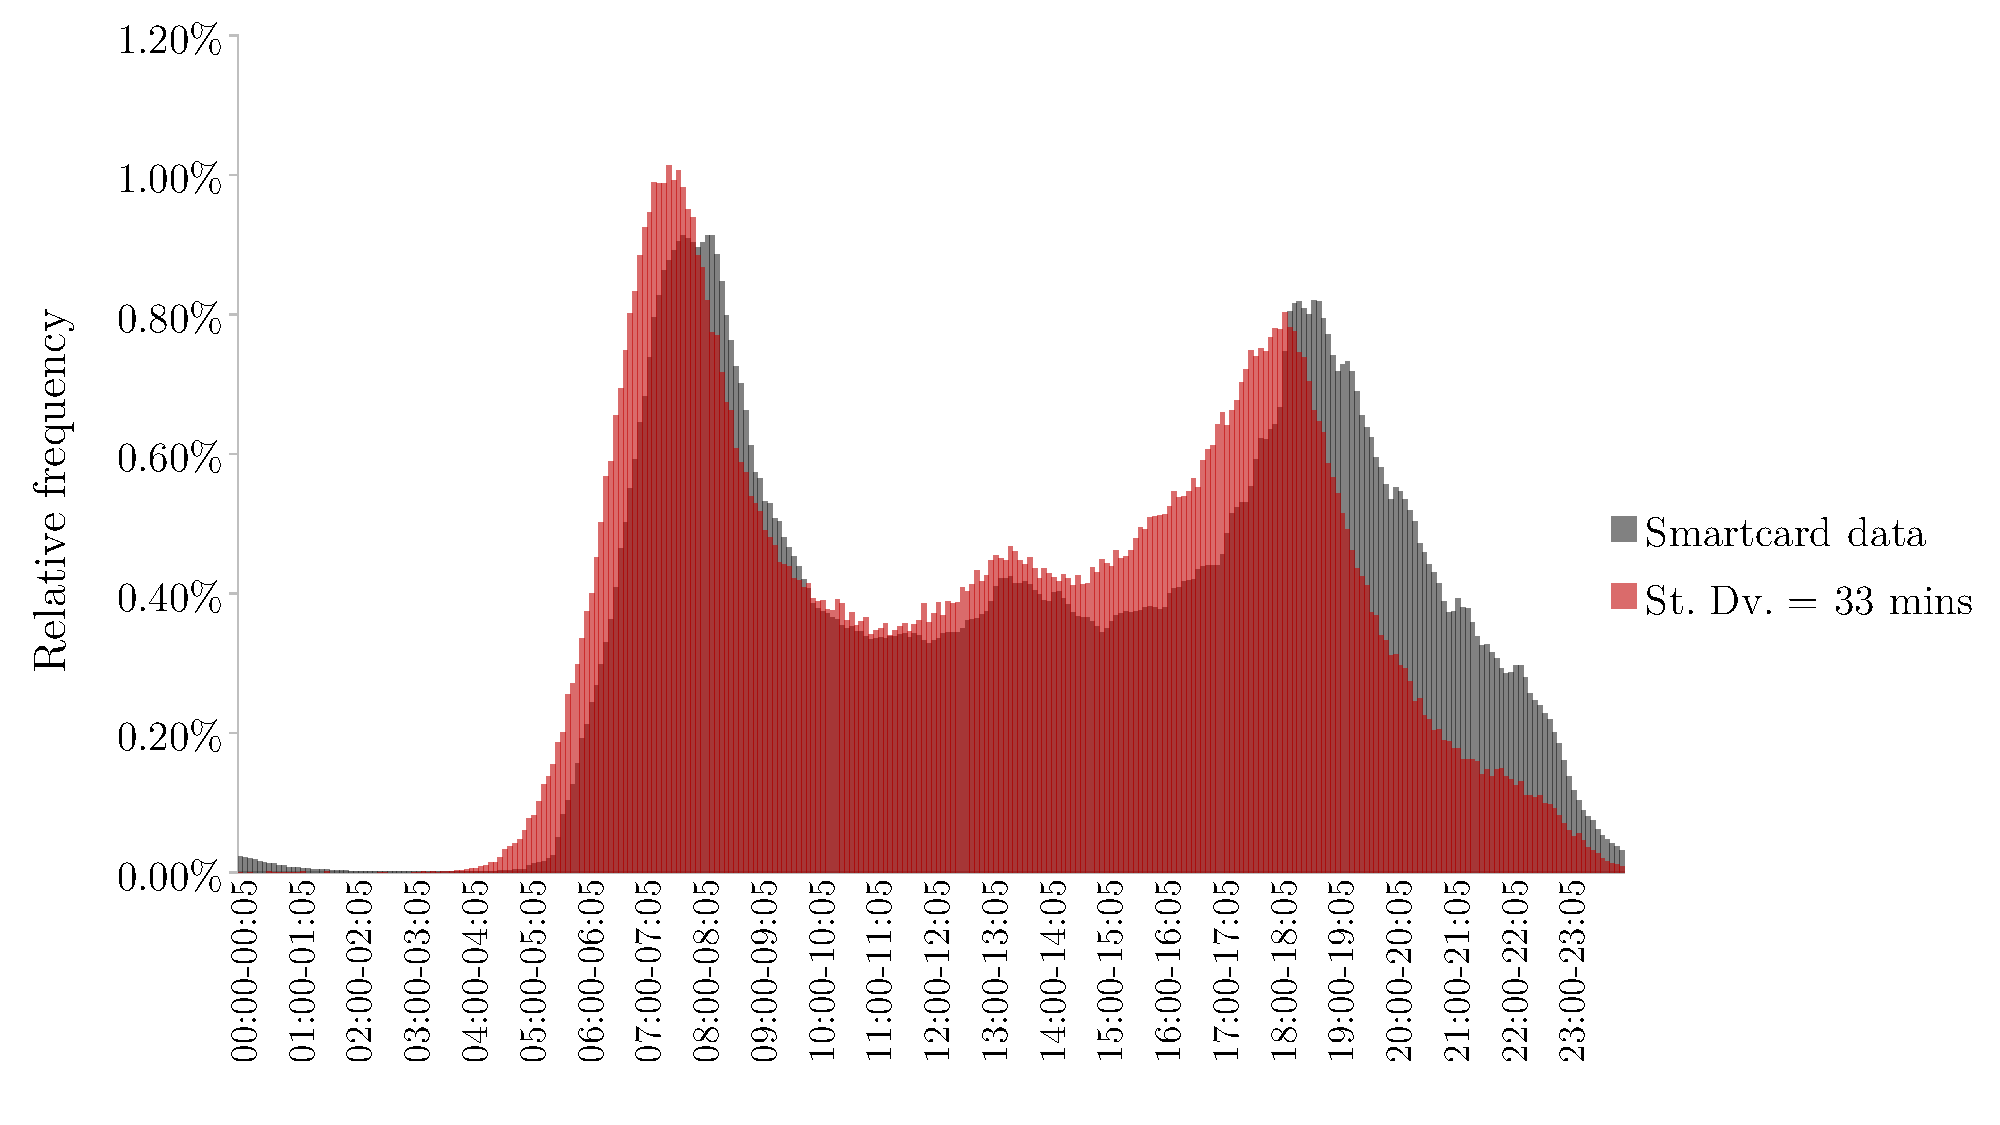
\includegraphics[scale=0.4]{images/1_CHI33SD.pdf}
    \caption{Comparison of randomized public transport trip start times with $\sigma_{\chi^2}^{*}=33$ minutes (in red) and smartcard data (in gray).}
    \label{histogram_comparition}
\end{figure}
%OK
The next step was to add variability to agents' activity locations. The goal in this case was to maintain as close as possible the observed land uses, assigning new activity locations to the cloned agents and maintaining the activity types considered in the original synthetic population (home, work, business, education, health, visit someone, shopping, leisure and other). An official land-registry from a Government institution (SII) was used to this end, which corresponds to a georeferenced data-set with the number of places/buildings by different categories in every block of the city\footnote{The number of places/buildings by block and the georeferenced data-set with the blocks information had to be merged previously to this step.} Blocks extending outside the main urban area were reduced before activity locations re-assignment process. Once already pre-processed, the georeferenced data-set was used to choose new coordinates for every activity of the cloned agents. In particular, new coordinates were chosen randomly based on the original activity type and inside the original traffic analysis zone, similar to the work made by \cite{kickhofer2013rising}. An example of the home activity location distribution before and after the randomization process can be seen in Figure \ref{homeDistribution}. This step ends up with a population denominated as $\pi_{10}^{f}$. Agents representing a $1\%$ of the Santiago's total population were randomly sampled from $\pi_{10}^{f}$ in order to obtain a more light-weight scenario to simulate, denominated $\pi_{1}^{f}$

\begin{figure}
	\centering
	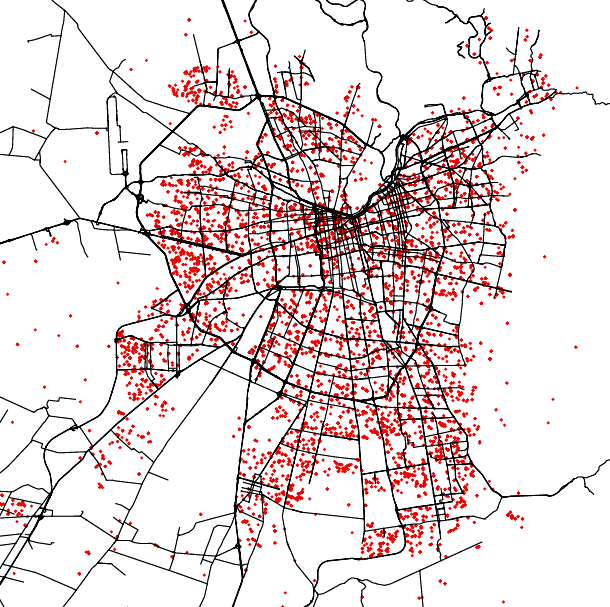
\includegraphics[width=.4\linewidth]{images/homeOriginal10AM.png}\hspace{1cm}
	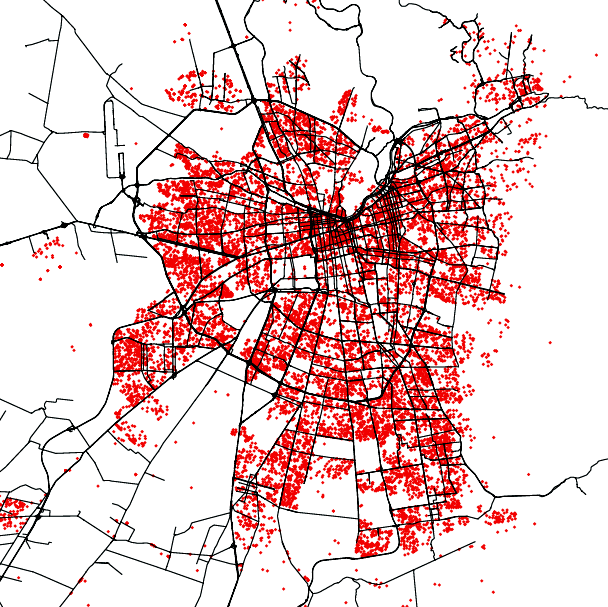
\includegraphics[width=.4\linewidth]{images/homeRandomized10AM.png}
	\caption{Home activity location at 10:00 AM. Left: Before randomization. Right: After randomization}
	\label{homeDistribution}
\end{figure}
%OK
The final step was the inclusion of tolls to the tollways already included in the scenario network. Information about 2012's tolls was gathered from different resources (Government Institutions such as Ministry of Public Works, Annual Reports from tollways' operators, and other online resources). Since not all the 2012's tolls were available, some of them were adjusted from the last available year to 2012 values, following the expression tollways operators used to update them in an annual basis.

In order to include the tolls in the scenario, a shape file was built with lines crossing the corresponding MATSim network links, which represent the gantries' approximate locations. Finally, the fares were included using the MATSim road pricing module \citep{RoadPricinginMATSim}, which applies the corresponding fares when agents enter the tolled links computing the term $\beta_{m}\cdot\Delta m_{q}$ in the performance function (See Eq. \ref{performanceTraveling}). This step ended the input improvement process, giving as a result the so-called \textit{improved-scenario}, which was the starting point to the calibration process, step that is necessary to ensure that the model is capable to replicate a set of observed conditions.


%\begin{itemize}
%    \item Expansion of synthetic population based on Contreras (2015): OK.
%    \item Randomization of activity start times: OK.
%    \item Randomization of activity locations: OK
%    \item Addition of tolls to tollways: OK
%    \item Some general conclusions and TO-DO's: OK
%\end{itemize}
%OK
\subsection{Calibration}

The main goal of the calibration process is to end up with a model able to replicate some predefined set of observed conditions, such as modal split, traffic flow or distributions of travel times and distances. In this work, the improved-scenario was calibrated to replicate the observed modal split and hourly traffic flow in specific counting stations distributed across the city \citep{AFOROS2013}. Different initial settings were explored with the $\pi_{1}^{f}$ population in order to know the simulator response with a light-weight scenario. The final initial setting was then applied to the scenario with the $\pi_{10}^{f}$ population.

The initial step in this process was to calibrate the modal split, which was achieved by changing the values of the Alternative Specific Constants (ASCs) iteratively based on the expression proposed by \cite{manski1977estimation}. Let $P_{obs}(m)$ be the observed modal split of mode $m$ in the ODS and $P_{n}^{s}(m)$ the corresponding modal split in MATSim after $n$ iterations for the $s_{th}$ simulation \footnote{Recall that a simulation is composed of multiple iterations}, then the correction of the corresponding ASC was made based on,
\begin{equation}
C_{m}^{s+1}=C_{m}^{s}-\ln\Bigg(\frac{P_{n}^{s}(m)}{P_{obs}(m)}\Bigg)
\end{equation}

Once the calibration of the ASCs was completed (i.e. when the simulated modal split of the calibrated modes where close enough to the observed modal splits), the traffic volumes were corrected using the \emph{Calibration of Dynamic Traffic Simulations} (Cadyts) tool (\cite{cadytsmanual}, \cite{flotterod2011bayesian},\cite{CaDyTS}). In short, let $y_{a}(k)$ be the observed traffic flow during hour $k$ in link $a$ and $q_{a}(k)$ the corresponding traffic flow in the simulation for the same hour and link. Also, let $\sigma_{a}^2(k)$ be the variance of the traffic counts. Then, it is possible to sample from a posterior route choice distribution given certain level of services and information of traffic counts modifying the prior distribution by adding terms to the scoring function given by\citep{flotterod2011bayesian},

\begin{equation}
\Delta S_{a}(k)=\frac{y_{a}(k)-q_{a}(k)}{\sigma^2_{a}(k)}
\end{equation}


Assuming that the random variable representing the traffic flow in link $a$ during hour $k$, $Y_{a}(k)$ follows a Poisson distribution with rate parameter $y_{a}(k)$, then its variance is assumed to be,
\begin{equation}
\label{modifiedVariance}
\sigma_{a}^2(k)=\lambda\cdot \max(y_{a}(k), \sigma^2_{min})
\end{equation}

which is a modification of the variance of a Poisson variable by a scale parameter $\lambda$ usually fixed at 1 and a $\sigma^2_{min}$ to avoid numerical issues \citep{flotterod2011bayesian}.

Finally, the modified agents' utility is given by,

\begin{equation}
\label{modifiedUtility}
\tilde{S}_{\mathit{i}}=S_{\mathit{i}}+w\sum_{ak\in \mathit{i}}\Delta S_{a}(k)
\end{equation}

where $i$ represents a particular plan, so the sum in (\ref{modifiedUtility}) is made over all the links and hours within plan $i$ that contain information about traffic counts, and $w$ is a weight parameter defined before Cadyts application. It is important to note that, since the scenarios are scaled in terms of the number of agents (1\% and 10\% of the real Santiago's population) the simulated traffic flows were amplified in order to be congruent with the magnitude of traffic counts.

When simulating large-scale scenarios, it is recommended to control the oscillations of agents' behavior between one iteration and the next \citep{MATSimSantiago}, which is achieved by controlling the re-planning step. In this work, the modal split calibration assumed that during the first 80\% of iterations within a simulation, 15\% of agents explore new routes, another 15\% explore new modes (between \emph{car}, \emph{public transport} y \emph{walk}) and the remaining 70\% choose between plans that were already explored in the past. During the final 20\% of iterations, the re-planning step was turned off, so agents can choose only between plans already existing in their memories, and forcing the convergence of scores through the method of successive averages (MSA). The plan selection by every agents is made assuming a changing-plan probability that depends on $\exp(\Delta_{score})$, where $\Delta_{score}$ is the difference between two plans scores \citep{ConfiguringMATSim}
%OK
Since the calibration of traffic volumes started from the iteration with calibrated modal splits, Cadyts was applied assuming that agents could re-plan only in terms of new routes. Similar to the modal split calibration process, the re-planning in this case was carried out only for the first 80\% of iterations, and then turned off for the final 20\%.

Two stability-simulations were run for 1\% and 10\% cases in order to check if changes made by the modal split and traffic volumes calibration processes were stable once Cadyts were turned off . The first stability-simulation (\emph{stability-test with innovation}) considered a re-planning where 15\% of agents were able to change between routes, another 15\% were able to explore new modes, and the remaining 70\% choose between plans already explored for the first 80\% of the iterations. For the final 20\% of the iterations, agents changed between already explored plans, and scores were averaged through MSA. The second stability-simulation (\emph{stability-test without innovation}) assumed no re-planning at all, so scores were averaged through MSA from the simulation start. Also, the 1\% Case was simulated from an increased number of iterations with the ASCs$^{*}$ already found in the modal-split calibration process in order to check the stability of this particular result (\emph{modal-split stability-test}).
%OK
\subsubsection{Calibration and stability tests results}
Tables \ref{table:modal_splits_1pct} and \ref{table:modal_splits_10pct} show the results of the modal-split calibration process for the 1 and 10\% cases. It is important to note that, in both scenarios, agents were able to choose only between car, public transport, and walk, so both observed and simulated modal splits were scaled up such that they add up 100\%. In both tables, subscripts denote the iteration number inside a given simulation, and superscripts denote the simulation number. In the 1\% case, the calibrated scenario was obtained for the 30th simulation, and in the 10\% it was obtained for the 7th one. The reference iteration to evaluate the modal splits and their similarity with the observed ones is iteration 100 for both cases.

\begin{table}
\caption{Alternative specific constants and modal splits for 1\% case.}
\begin{tabular}{c|c|cc|cc}
\hline
Modo                      &$\tilde{P}_{obs}(m)$ [\%]& $ASC^{0}(m)$	& $\tilde{P}_{50}^{0}(m)$ [\%]	& $ASC^{*}(m)$& $\tilde{P}_{100}^{*}(m)$ [\%]\\
\hline
\emph{Car}             	  & 30,164 & 0,000 & 22,829 & 1,265  & 30,811 \\
\emph{Public Transport}   & 29,343 &-1,058 & 35,344 & -0,695 & 28,187 \\
\emph{Walk}               & 40,493 &-0,143 & 41,827 & -1,183 & 41,002 \\
\hline
\end{tabular}
\label{table:modal_splits_1pct}
\end{table}

\begin{table}
	\caption{Alternative specific constants and modal splits for 10\% case.}
	\begin{tabular}{c|c|cc|cc}
		\hline
		Modo                      &$\tilde{P}_{obs}(m)$ [\%]& $ASC^{0}(m)$	& $\tilde{P}_{50}^{0}(m)$ [\%]	& $ASC^{*}(m)$& $\tilde{P}_{100}^{*}(m)$ [\%]\\
		\hline
		\emph{Car}             	  & 30,164 & 0,000 & 24,762 & 0,838  & 29,624 \\
		\emph{Public Transport}   & 29,343 &-1,058 & 34,263 & -1,676 & 29,331 \\
		\emph{Walk}               & 40,493 &-0,143 & 40,975 & -0,254 & 41,045 \\
		\hline
	\end{tabular}
\label{table:modal_splits_10pct}
\end{table}
%OK
For the traffic volumes calibration, Cadyts was applied in both 1\% and 10\% during $n_{c}=500$ iterations from iteration 100 (which corresponds to the modal-split calibrated scenario). The parameters $\lambda$, $\sigma^{2}_{min}$ of Equation \ref{modifiedVariance} and $w$ of Equation \ref{modifiedUtility} were maintained with their default values of $\lambda=1$, $\sigma^{2}_{min}=25^2$ [veh/h]$^2$ and $w=30$. The results are shown graphically in Figures \ref{fig:obs_vs_sim_1pct} and \ref{fig:obs_vs_sim_10pct} for the 1\% and 10\% case, respectively.

\begin{figure}[h!]
	\centering
	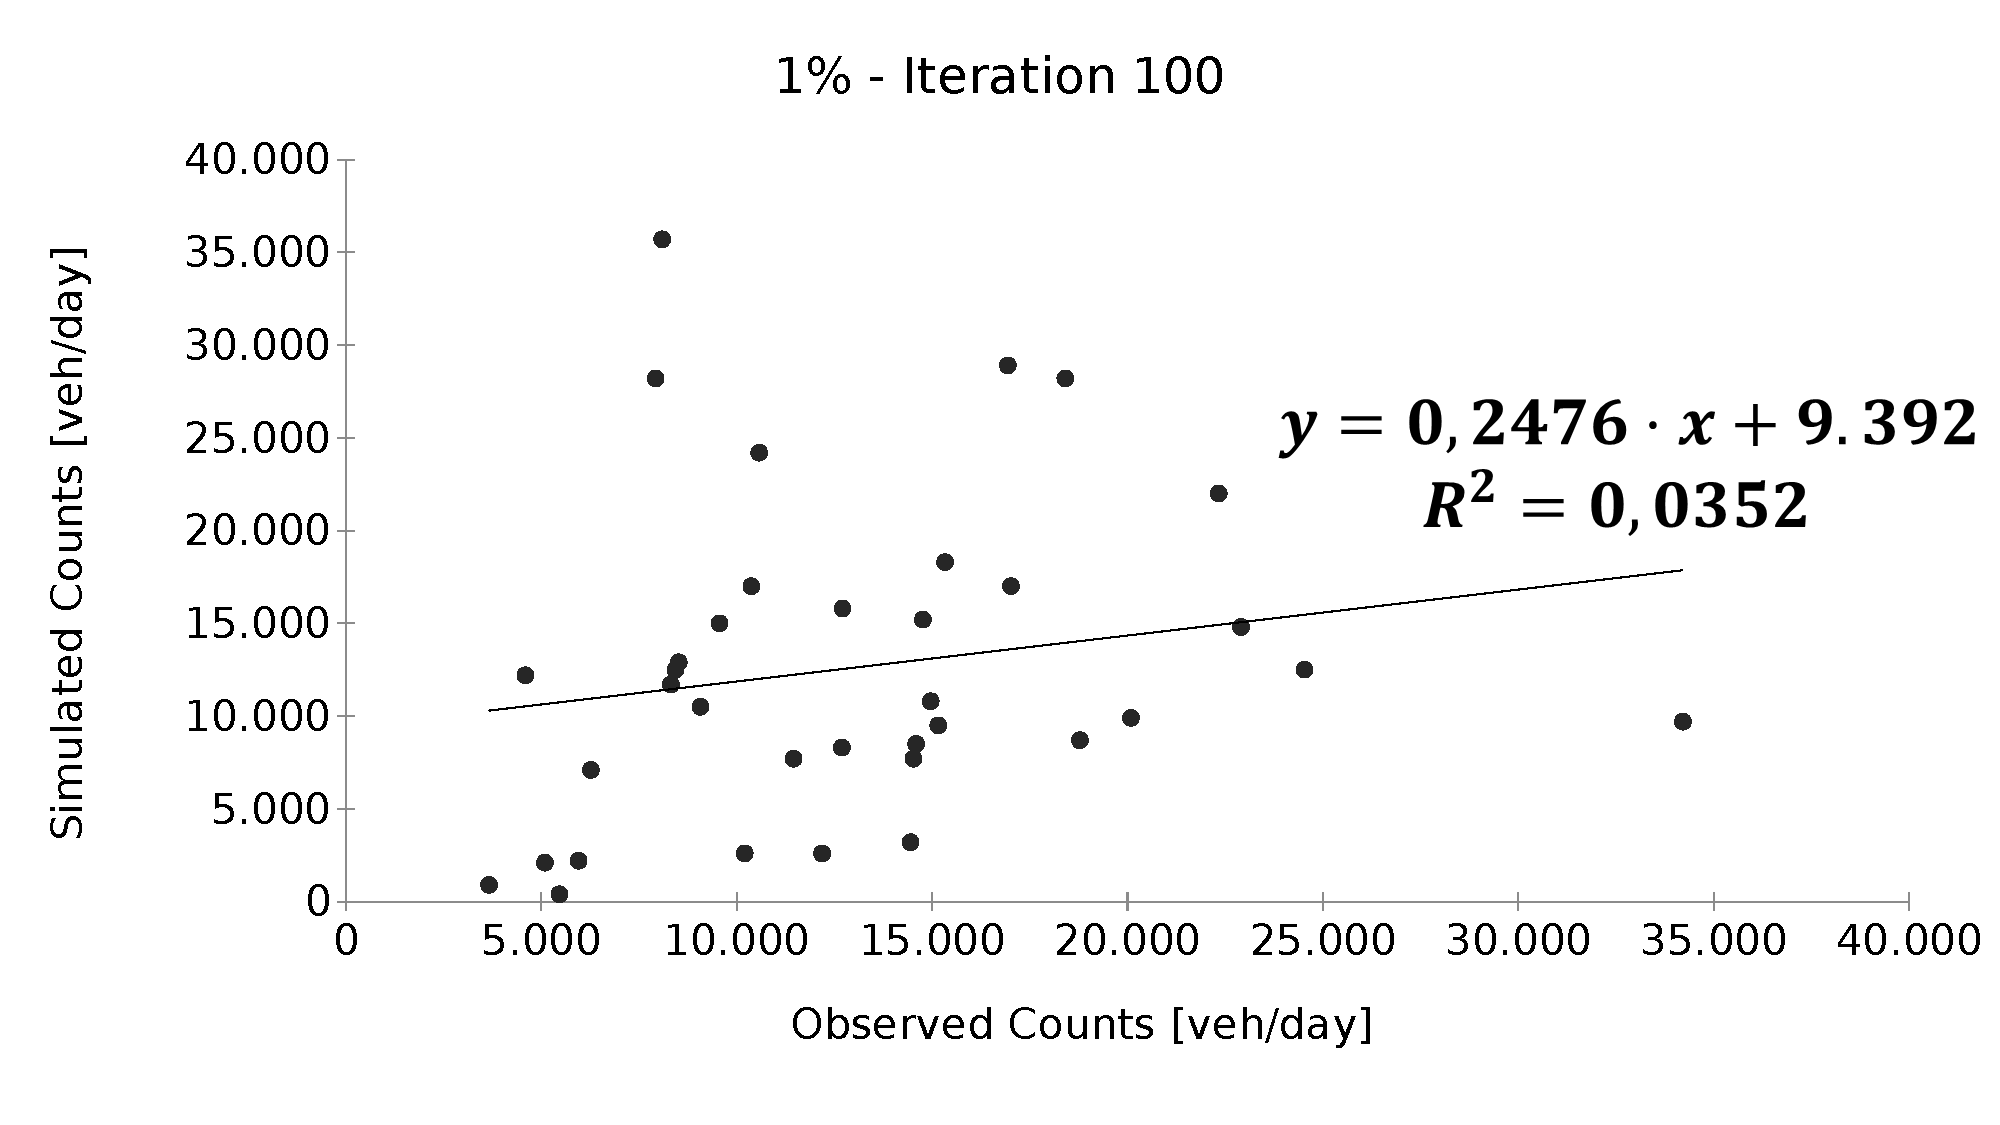
\includegraphics[scale=0.22]{images/1pct_it100.pdf}\hspace{1cm}
	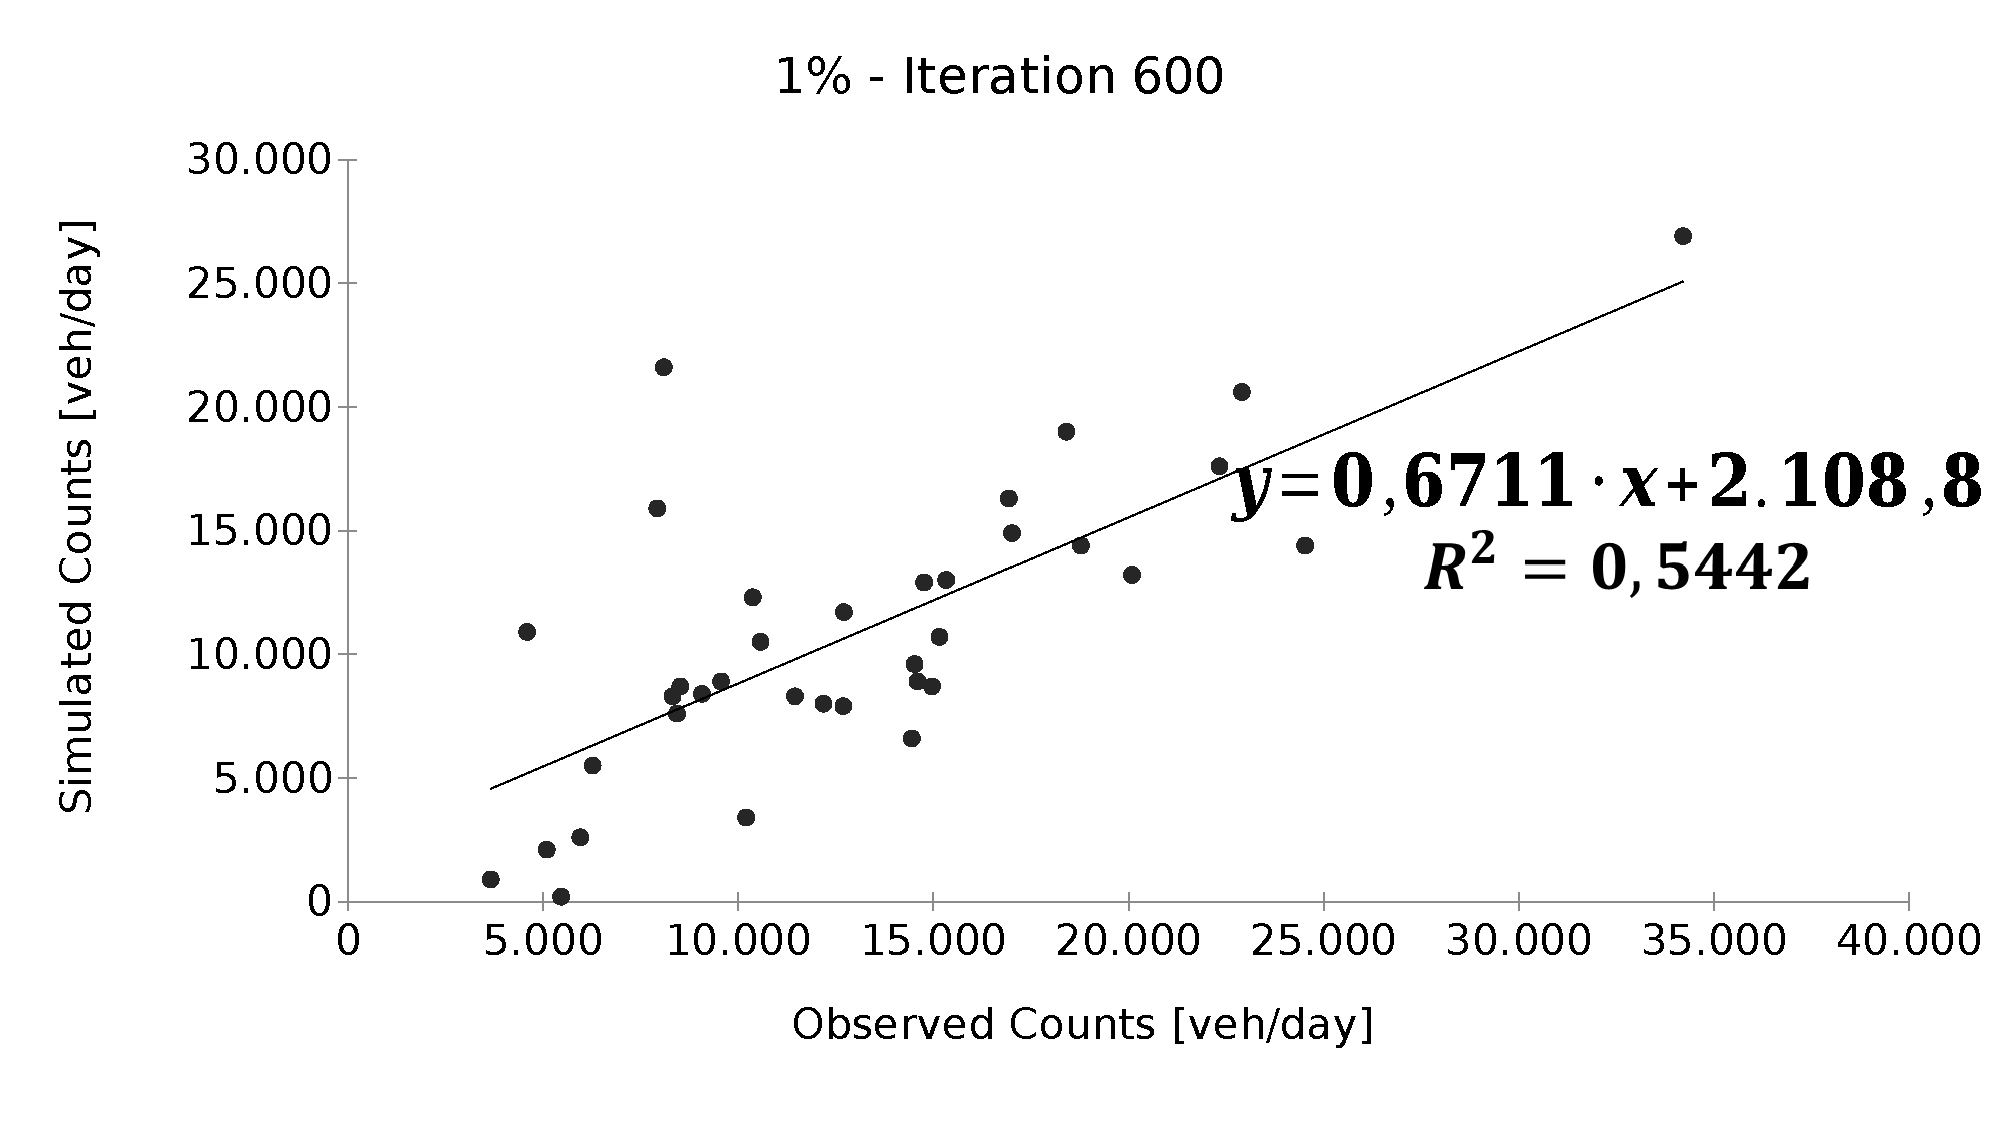
\includegraphics[scale=0.22]{images/1pct_it600.pdf}
	\caption{Observed vs. simulated counts for 1\% case. Left: Before Cadyts application. Right: After Cadyts application}
	\label{fig:obs_vs_sim_1pct}
\end{figure}

\begin{figure}[h!]
	\centering
	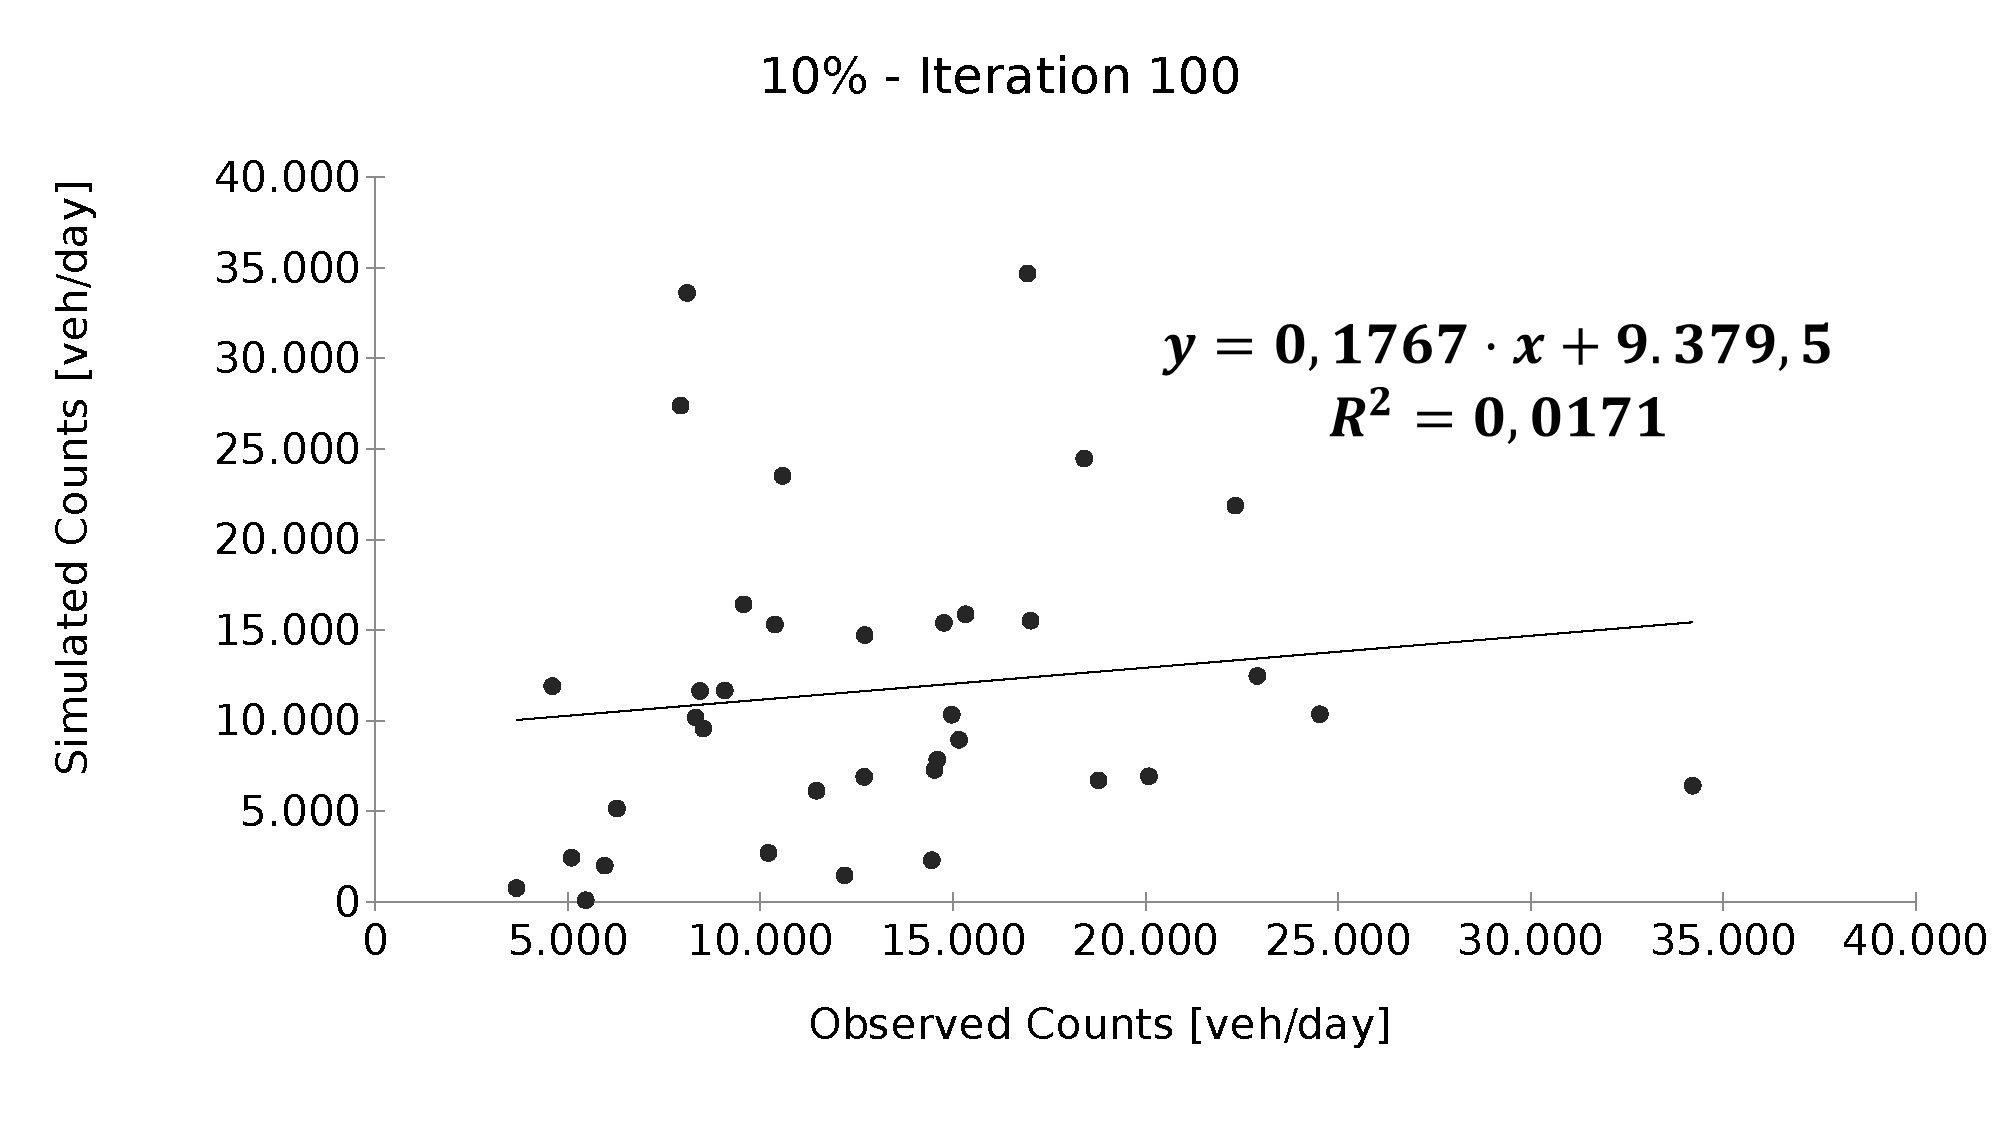
\includegraphics[scale=0.22]{images/10pct_it100.pdf}\hspace{1cm}
	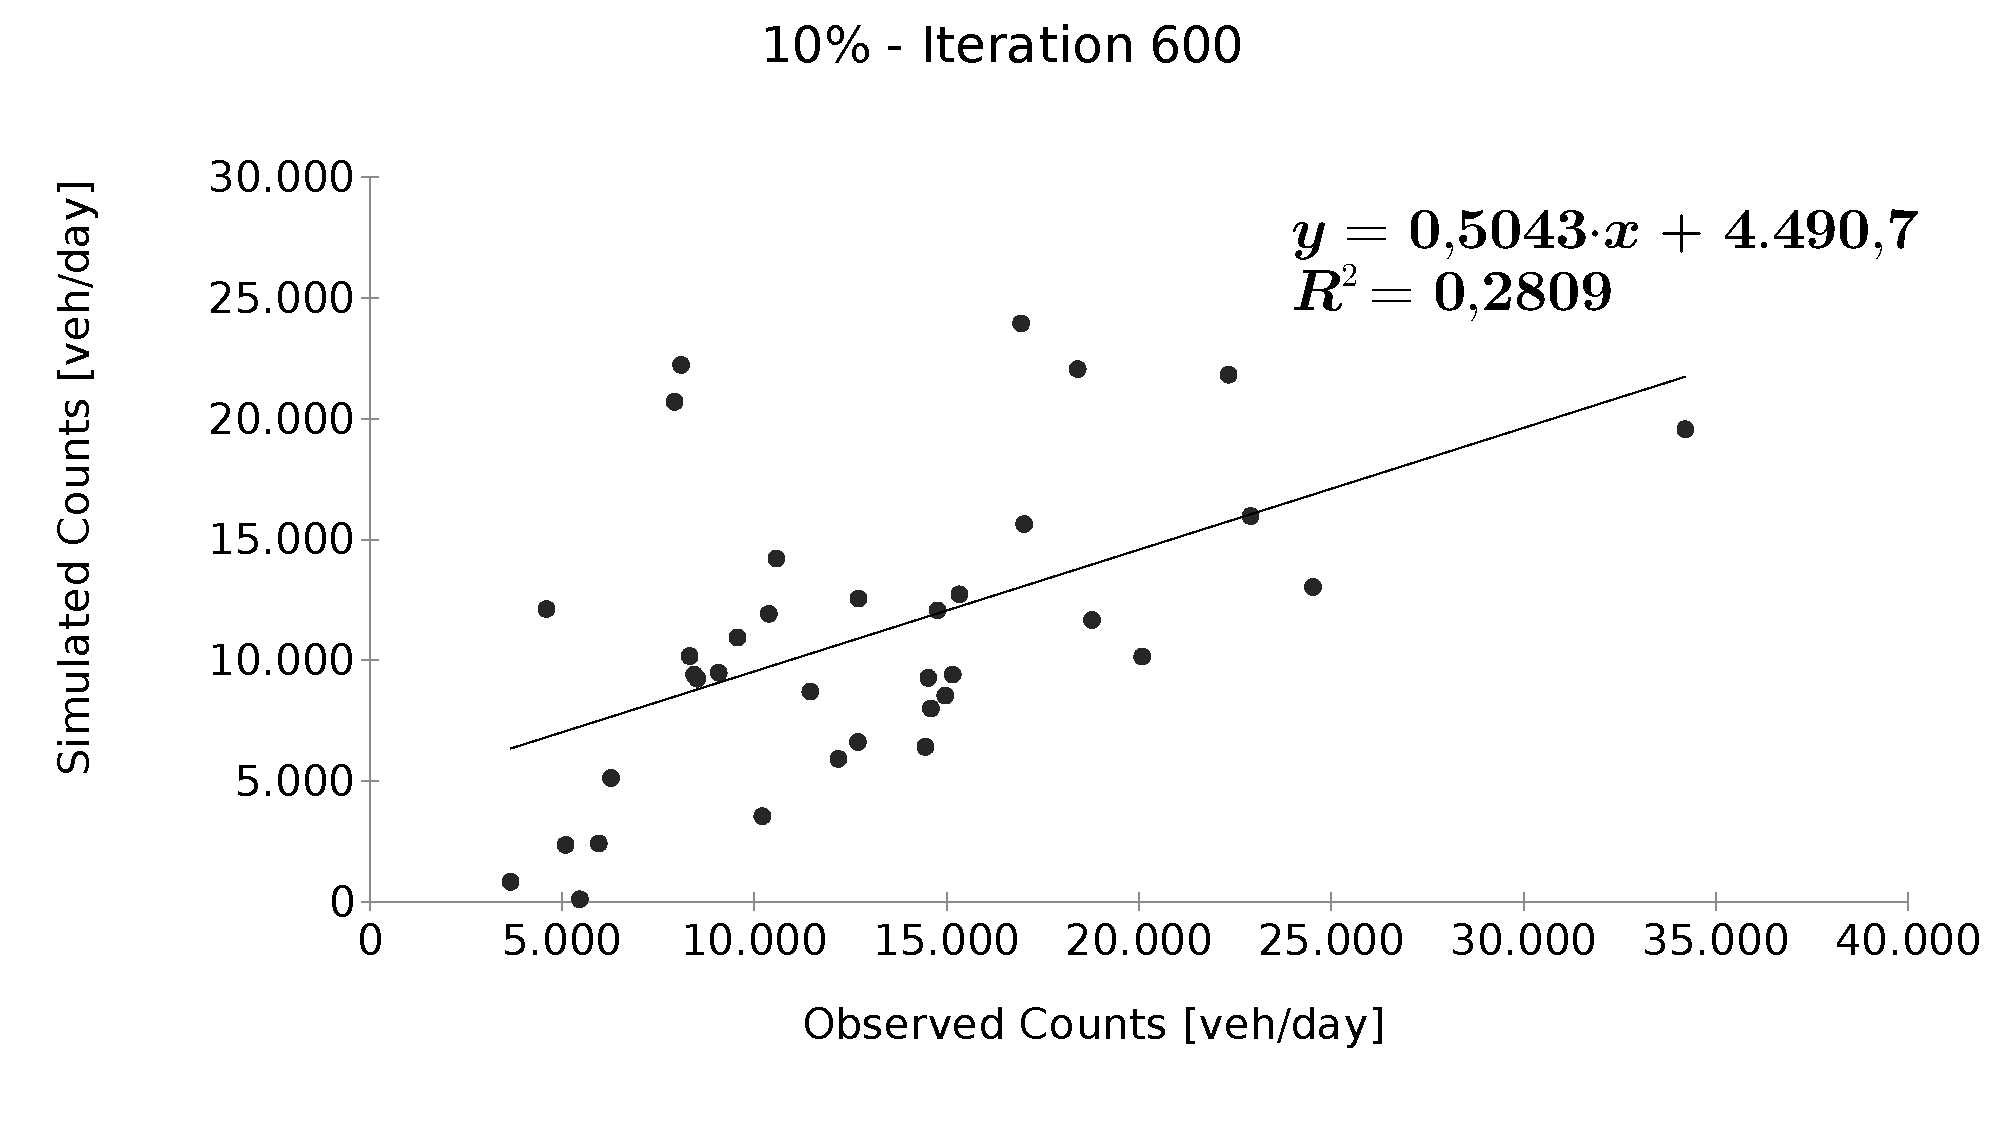
\includegraphics[scale=0.22]{images/10pct_it600.pdf}
	\caption{Observed vs. simulated counts for 10\% case. Left: Before Cadyts application. Right: After Cadyts application}
	\label{fig:obs_vs_sim_10pct}
\end{figure}
%Figure of hourly GEH for it 100 and 600 for 1% and 10%?
%OK
In terms of stability, Table \ref{table:1pct_modalSplitEvolution} shows the evolution of modal splits through the final iterations for the 1\% case. The modal-split stability-test corresponds to a $n_{e1}=500$ iterations simulation starting from iteration 0 with ASCs$^{*}$ The stability-test with and without innovations corresponds to a $n_{e2}=200$ iterations simulations starting from iteration 600 (modal-split and traffic volumes calibrated scenario).

\begin{table}
	\caption{Modal split evolution of car mode through the final iterations for the 1\% case.}
	\label{table:1pct_modalSplitEvolution}
	\begin{tabular}{ccccc}
		\hline	
		Scenario & Iteration & $\tilde{P}_{n}(car)$ [\%] &  $\tilde{P}_{n}(PT)$ [\%]&$\tilde{P}_{n}(walk)$ [\%] \\
		\hline
		Modal-split calibrated						& 100 & 30,811 & 28,187 & 41,002 \\
		Modal-split stability-test					& 500 & 31,596 & 27,810 & 40,594 \\
		Modal-split and traffic volumes calibrated	& 600 & 30,428 & 28,767 & 40,805 \\
		Stability-test with innovation				& 800 & 31,424 & 27,985 & 40,591 \\
		Stability-test without innovation			& 800 & 30,437 & 28,760 & 40,802 \\
		\hline
	\end{tabular}
\end{table}

Similarly, Table \ref{table:10pct_modalSplitEvolution} shows the evolution of modal splits through the final iterations for the 10\% case. In this case, no modal-split stability-test was run since it was assumed a similar response to the 1\% case from the simulator.

\begin{table}
	\caption{Modal split evolution of car mode through the final iterations for the 10\% case.}
	\label{table:10pct_modalSplitEvolution}
	\begin{tabular}{ccccc}
		\hline	
		Scenario & Iteration & $\tilde{P}_{n}(car)$ [\%] &  $\tilde{P}_{n}(PT)$ [\%]&$\tilde{P}_{n}(walk)$ [\%] \\
		\hline
		Modal-split calibrated						& 100 & 29,624 & 29,331 & 41,045 \\
		Modal-split and traffic volumes calibrated	& 600 & 29,548 & 29,749 & 40,702 \\
		Stability-test with innovation				& 800 & 30,333 & 29,113 & 40,554 \\
		Stability-test without innovation			& 800 & 29,559 & 29,738 & 40,703 \\
		\hline
	\end{tabular}
\end{table}

%Talk about the similarity of modal splits between different scenarios in both 1% and 10% cases.
Observing the previous tables, it can be seen that the modal-split behavior is stable throughout the different simulations in both the 1\% and 10\% cases, in spite of the agents' utility modification made by Cadyts in between. In general, it can be assumed that the iteration 100 is sufficiently representative in terms of modal splits, such that a higher number of iterations will not affect significantly the modal splits given the simulator set-up used in this work. %Talk about the max. variation between modal splits in each case.
%OK
To summarize how close the simulated and observed counts are, Table \ref{table:1pct_fitEvolution} and \ref{table:10pct_fitEvolution} show the linear regression parameters built considering the observed counts and simulated counts as the independent and dependent variable, respectively, for the 1\% and 10\% cases (intercept, slope and R$^2$ statistic).

\begin{table}
	\caption{Linear regression parameters evolution through the final iterations for the 1\% case.}
	\label{table:1pct_fitEvolution}
	\begin{tabular}{ccccc}
		\hline	
		Scenario & Iteration & Intercept &  Slope & R$^{2}$ statistic \\
		\hline
		Modal-split calibrated						& 100 & 9.392,0  & 0,25 & 0,04 \\
		Modal-split stability-test					& 500 & 10.634,7 & 0,14 & 0,01 \\
		Modal-split and traffic volumes calibrated	& 600 & 2.108,8  & 0,67 & 0,54 \\
		Stability-test with innovation				& 800 & 9.981,3  & 0,19 & 0,02 \\
		Stability-test without innovation			& 800 & 4.263,4  & 0,41 & 0,26 \\
		\hline
	\end{tabular}
\end{table}

\begin{table}
	\caption{Linear regression parameters evolution through the final iterations for the 10\% case.}
	\label{table:10pct_fitEvolution}
	\begin{tabular}{ccccc}
		\hline	
		Scenario & Iteration & Intercept &  Slope & R$^{2}$ statistic \\
		\hline
		Modal-split calibrated						& 100 & 9.379,5  & 0,18 & 0,02 \\
		Modal-split and traffic volumes calibrated	& 600 & 4.490,7  & 0,50 & 0,28 \\
		Stability-test with innovation				& 800 & 10.014,9 & 0,10 & 0,01 \\
		Stability-test without innovation			& 800 & 5.661,7  & 0,36 & 0,14 \\
		\hline
	\end{tabular}
\end{table}

In the case of traffic volume calibration, both Table \ref{table:1pct_fitEvolution} and \ref{table:10pct_fitEvolution} show (1) an over-estimation of traffic volumes by the simulator when observed traffic counts are 0 since intercepts are all greater than $2.000$ veh/day and (2) a systematic under-estimation of traffic volumes since the slope coefficients are all lesser than 1. In both cases, it can be seen the effect of Cadyts in the three linear regression parameters, making intercepts decrease towards zero, slopes increase towards 1, and increasing the $R^2$ statistic. The \emph{stability-test with innovation} shows, however, that the simulator behavior once Cadyts is turned off, does not persist. This happens because changes made by including adding terms in the agents' utility function are erased once Cadyts is turned off.
%OK
\section{Illustration: Scaling effect and Policy Analysis}
%Travel times
%Travel distances.
After the calibration process, the scenarios were useful to make policy analyses. Also, since this work considered synthetic populations representative of the 1\% and 10\% of the Santiago's population, they were also useful to test the scaling effect in the simulation.
\subsection{Scaling effect}
\label{sect:scaling_effect}
1\% and 10\% calibrated scenarios were compared in terms of distance and travel times distributions made by car mode\footnote{pt and walk mode analyses were neglected since those modes were not simulated in the road network}. Relative frequency histograms were built with data of the 24 hours, filtering those trips with null travel times or distances, shown in Figure \ref{fig:times_distance_comparison}. 

\begin{figure}[h!]
	\begin{subfigure}{.5\linewidth}
		\centering
		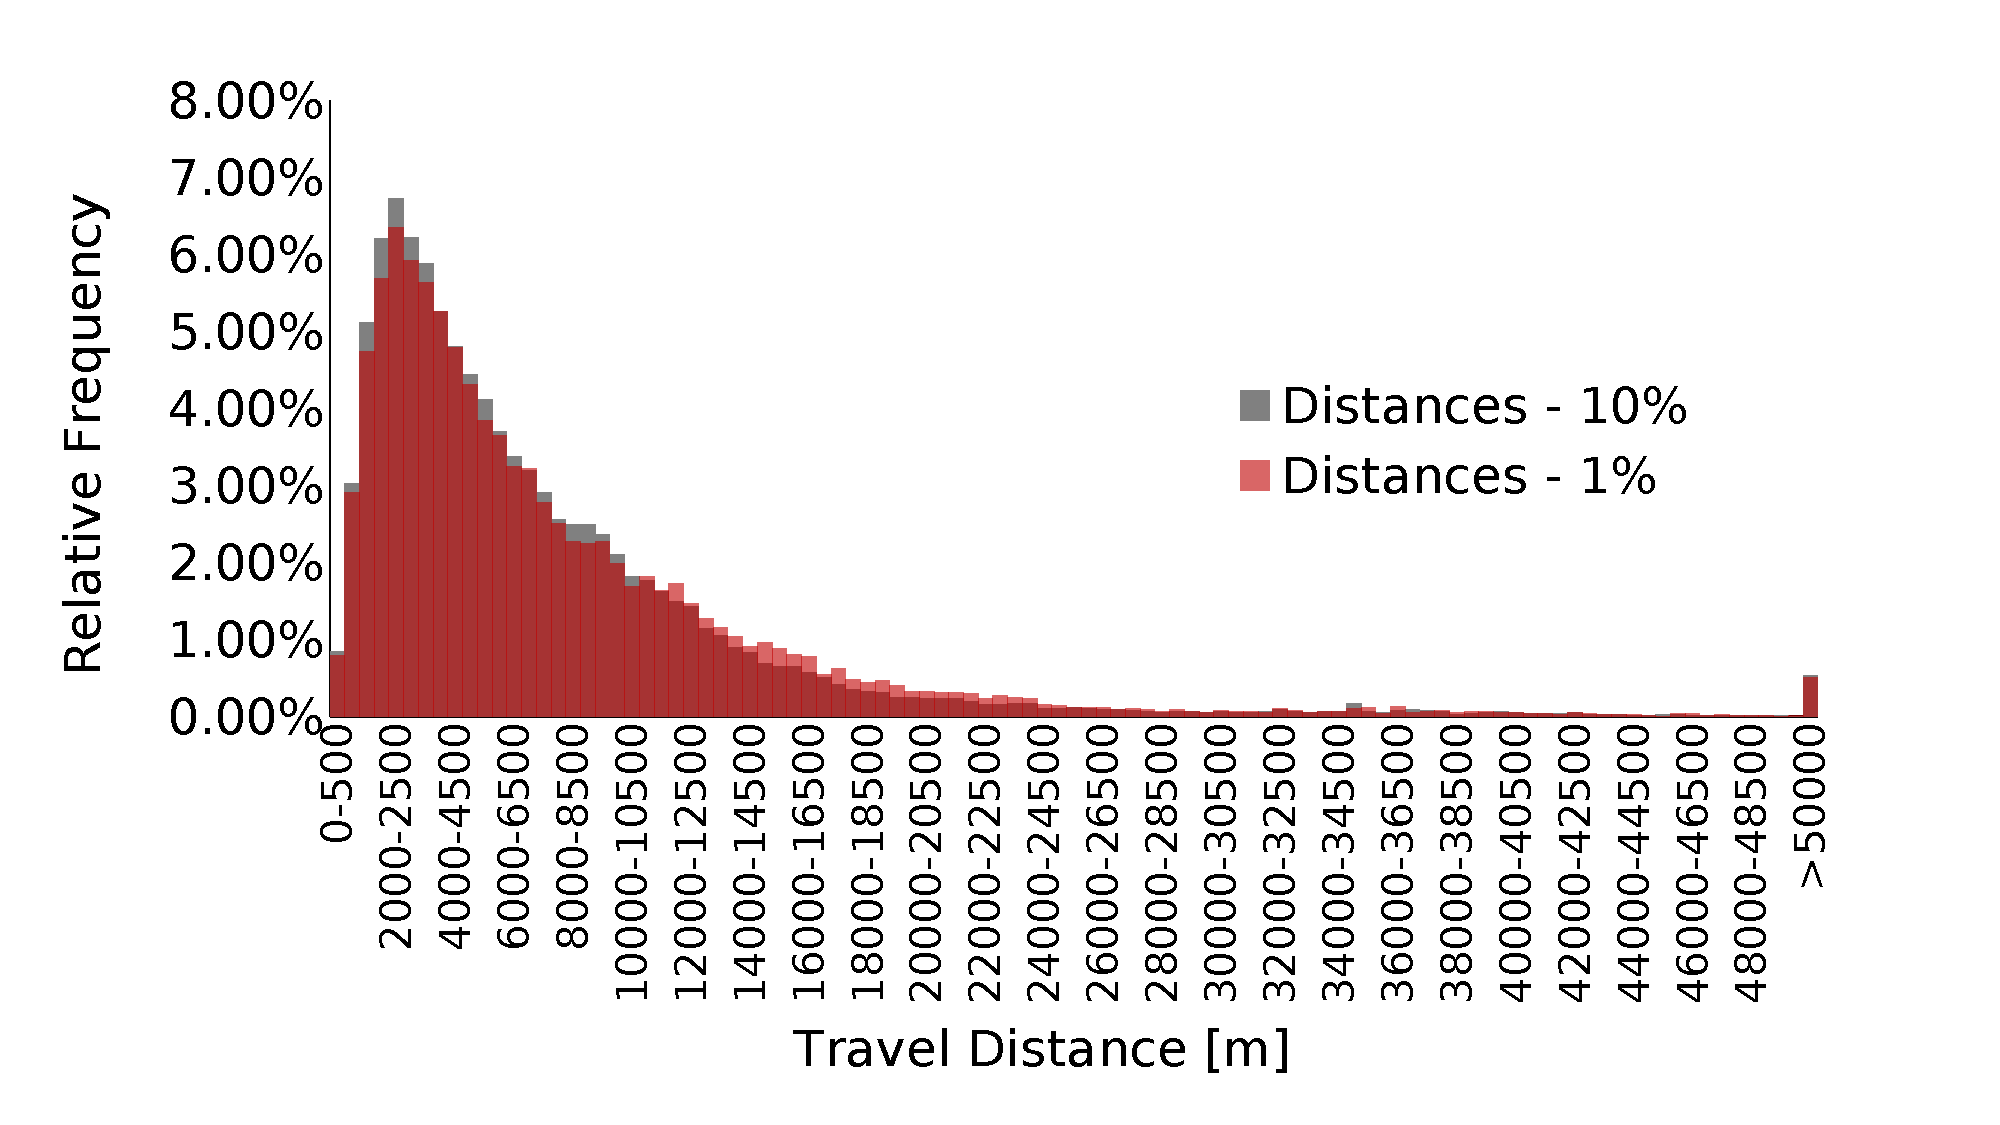
\includegraphics[scale=.25]{images/calibratedDistancesComparison.pdf}
		\caption{Traveled distances - Calibrated Scenario}
	\end{subfigure}%
	\begin{subfigure}{.5\linewidth}
		\centering
		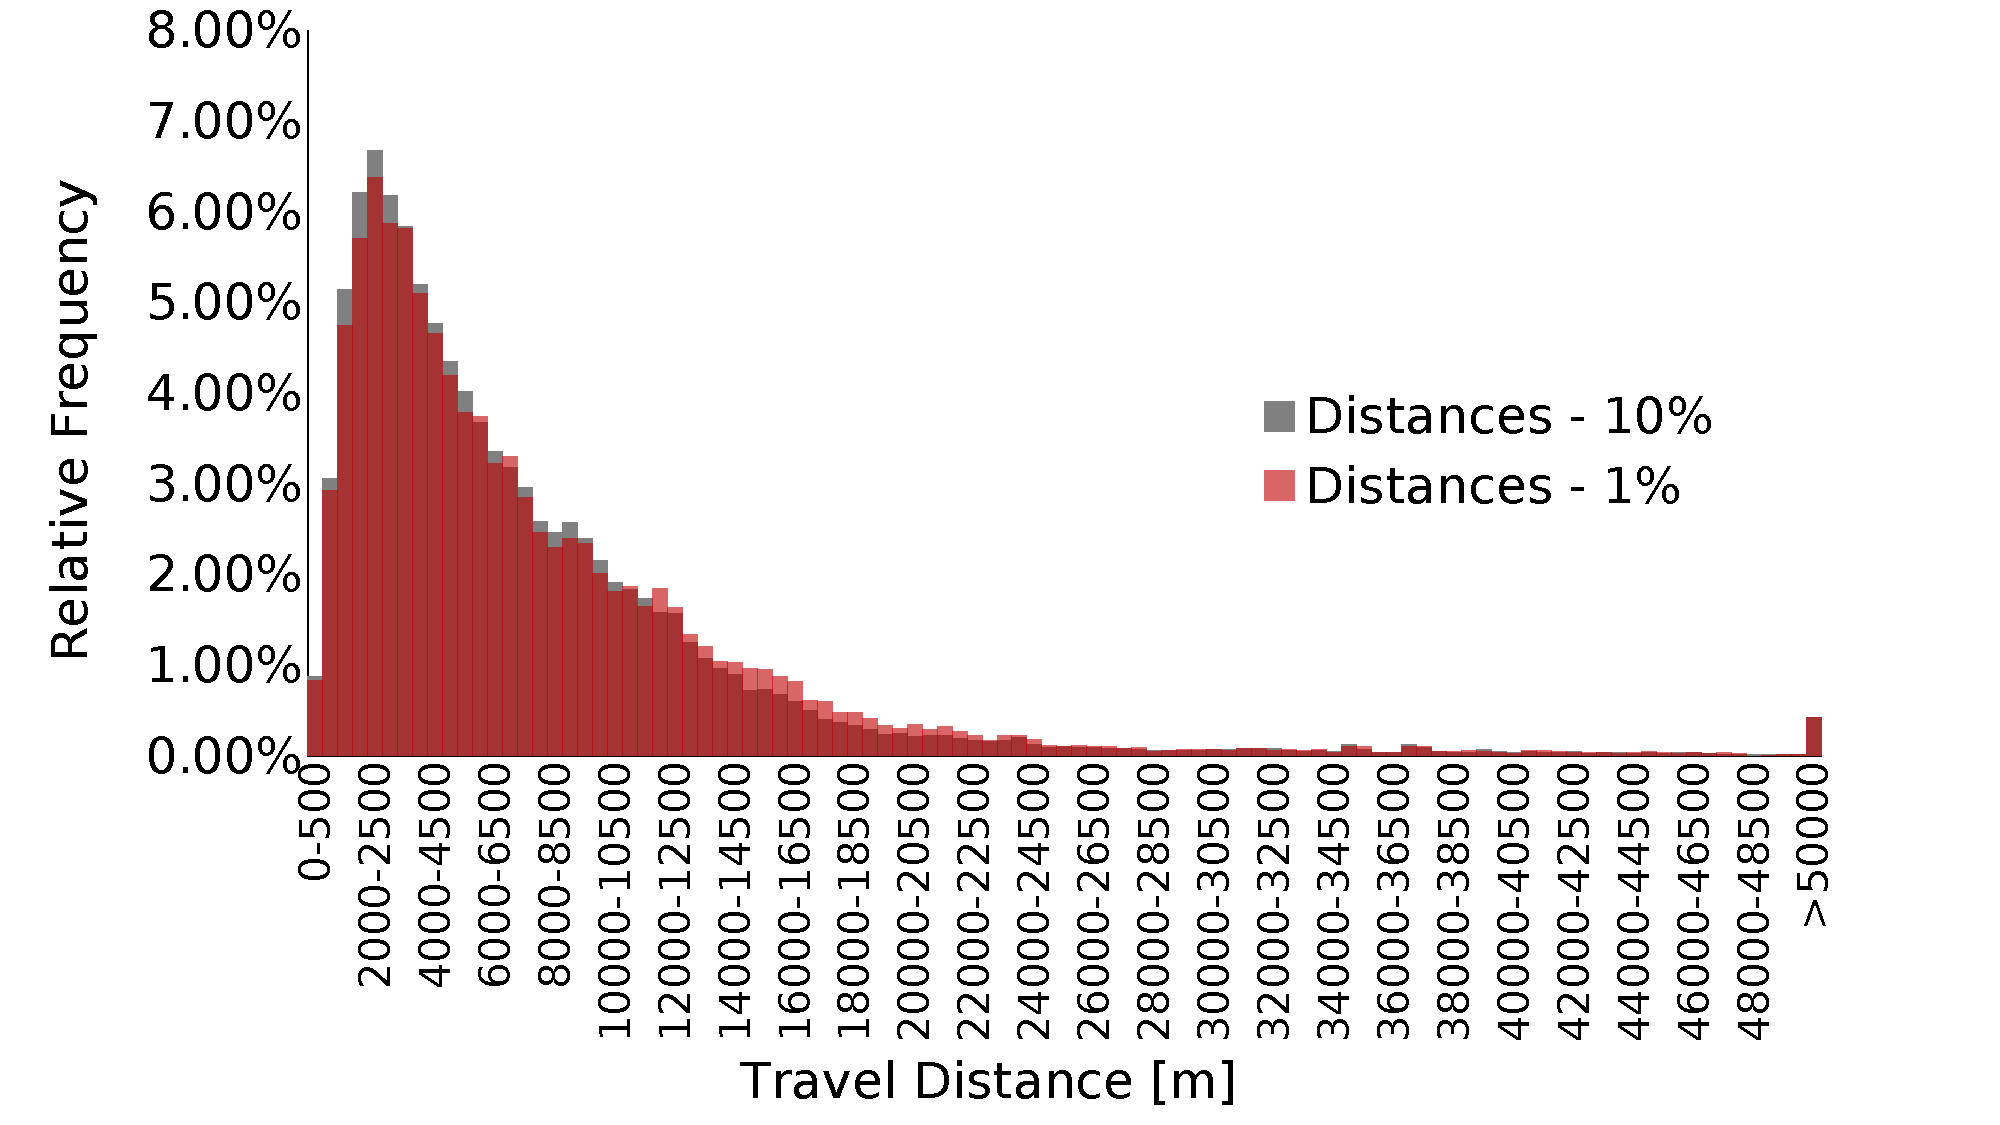
\includegraphics[scale=.25]{images/innovacionDistancesComparison.pdf}
		\caption{Traveled distances - Stability-test with innovation Scenario}
	\end{subfigure}\\[1ex]
	\begin{subfigure}{\linewidth}
		\centering
		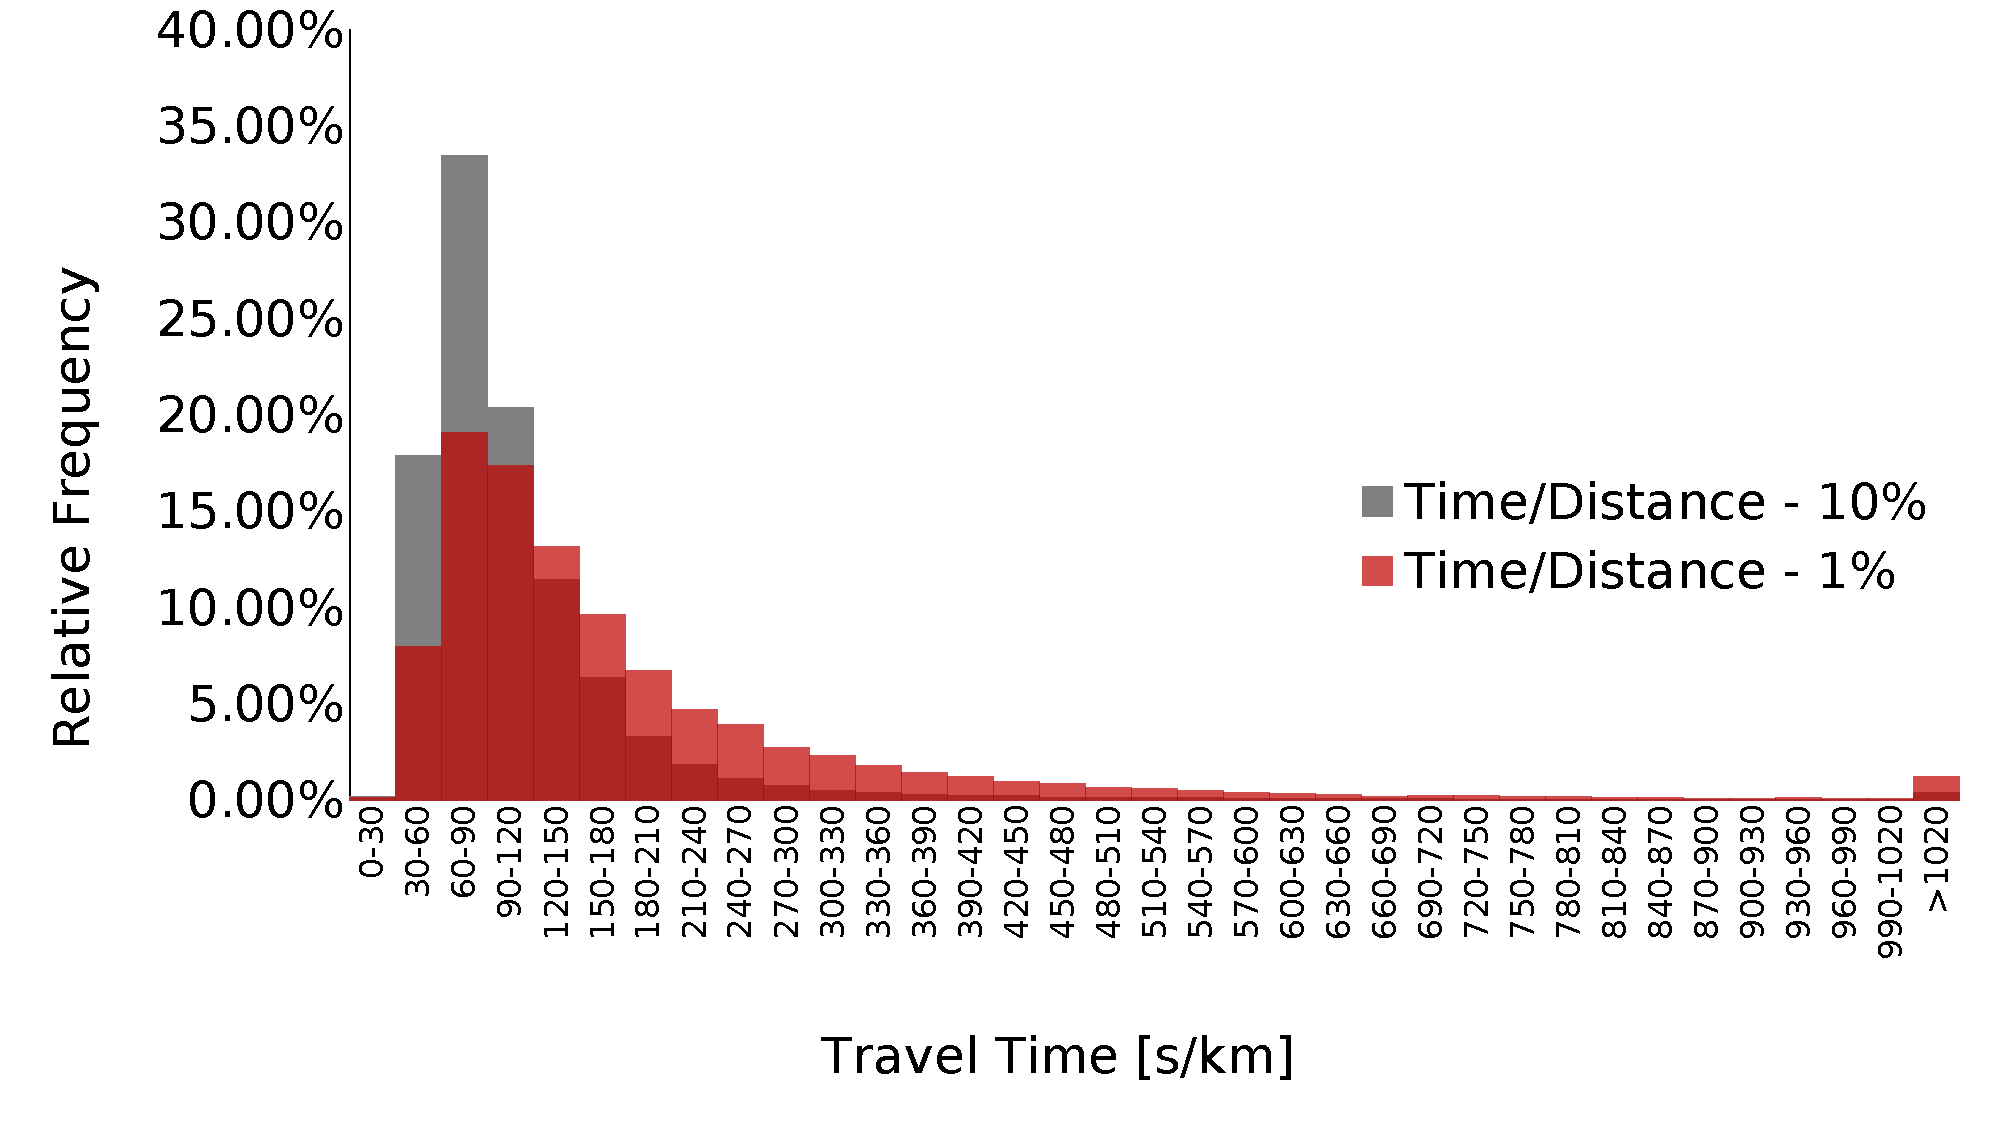
\includegraphics[scale=.3]{images/calibratedTimesComparison.pdf}
		\caption{Travel times - Calibrated Scenario}
	\end{subfigure}
	\caption{Traveled distances and times distributions}
	\label{fig:times_distance_comparison}
\end{figure}

Observing the traveled distances distribution, it can be seen that there is no notable difference between 1\% and 10\% cases, which can be interpreted as no effect in the assignment-step attributable to the scenario scaling. Traveled distances distribution for the Stability-test with innovation Scenario was also built to ensure that this conclusion was not dependent on Cadyts effect (see Figure \ref{fig:times_distance_comparison}, (a) and (b)). These figures validate the use of this type of scaling in MATSim scenarios for travel distances analyses, although a more rigorous statistical tests should be carried out to ensure this conclusion.
The above conclusion does not hold for the travel times. Observing Figure \ref{fig:times_distance_comparison}, (c), it can be seen that, in general, travel times for the 1\% case are greater than the ones for the 10\% case. This phenomenon occur due to the link capacities scaling method, where real capacities are multiplied by a scaling factor equals to the synthetic population sample rate. In the 1\% case, capacities were scaled down to their 1\%, affecting most importantly to links with small capacities. In particular, a great reduction in link capacities creates an over-estimation of the travel times, since a small amount of vehicles entering those small-capacity links create false congestion effects. This poses a warning in utilizing scenarios with a reduced number of agents ($<=1\%$) and scaled using the method presented in this work, if one wants to use the scenario to travel time analyses.
%OK
\subsection{Evaluation of a congestion pricing scheme}

The Calibrated Scenarios were used to evaluate a particular congestion pricing scheme and the results were compared with those obtained by \cite{gleave2009tarificacion} using the classical transport modeling approach in order to asses the level of sensitivity of the agent-based model used in this work.
%OK
\subsubsection{Schemes description}
The types of schemes considered in this work are cordon-based, such as the ones highlighted in Figure \ref{fig:congestion_pricing_schemes}. These schemes were originally proposed and evaluated by \cite{gleave2009tarificacion} using the ESTRAUS model \citep{ESTRAUS}, applied in its \emph{modal split - assignment} modality, meaning that the model considered changes in trip modes, routes and start times. The schemes were actively applied between 07:30 and 10:00 (morning peak, MP) and between 18:00 and 20:00 (evening peak, EP). The scenario used in that case was representative of 2015. The entry-link charge was defined first since vehicles using those links were considered to increase the congestion level inside the cordon. Exit-link charge was calculated proportionally to the ratio between exit and entry flow in the base case scenario. Users traveling inside the area were not charged at all. 
%OK
Given this input information, the charges used in the present work were the highest ones proposed in the reference study (see Table \ref{table:cordon_charges}). Simulations of 200 iterations were run from Calibrated Scenarios considering the (a) Outer cordon and (b) Triangle cordon schemes, whose results were compared with the Stability-test with innovation scenario, which represents the \emph{business as usual} case. This comparison was made for the 1\% and 10\% cases.

\begin{figure}[h!]
	\centering
	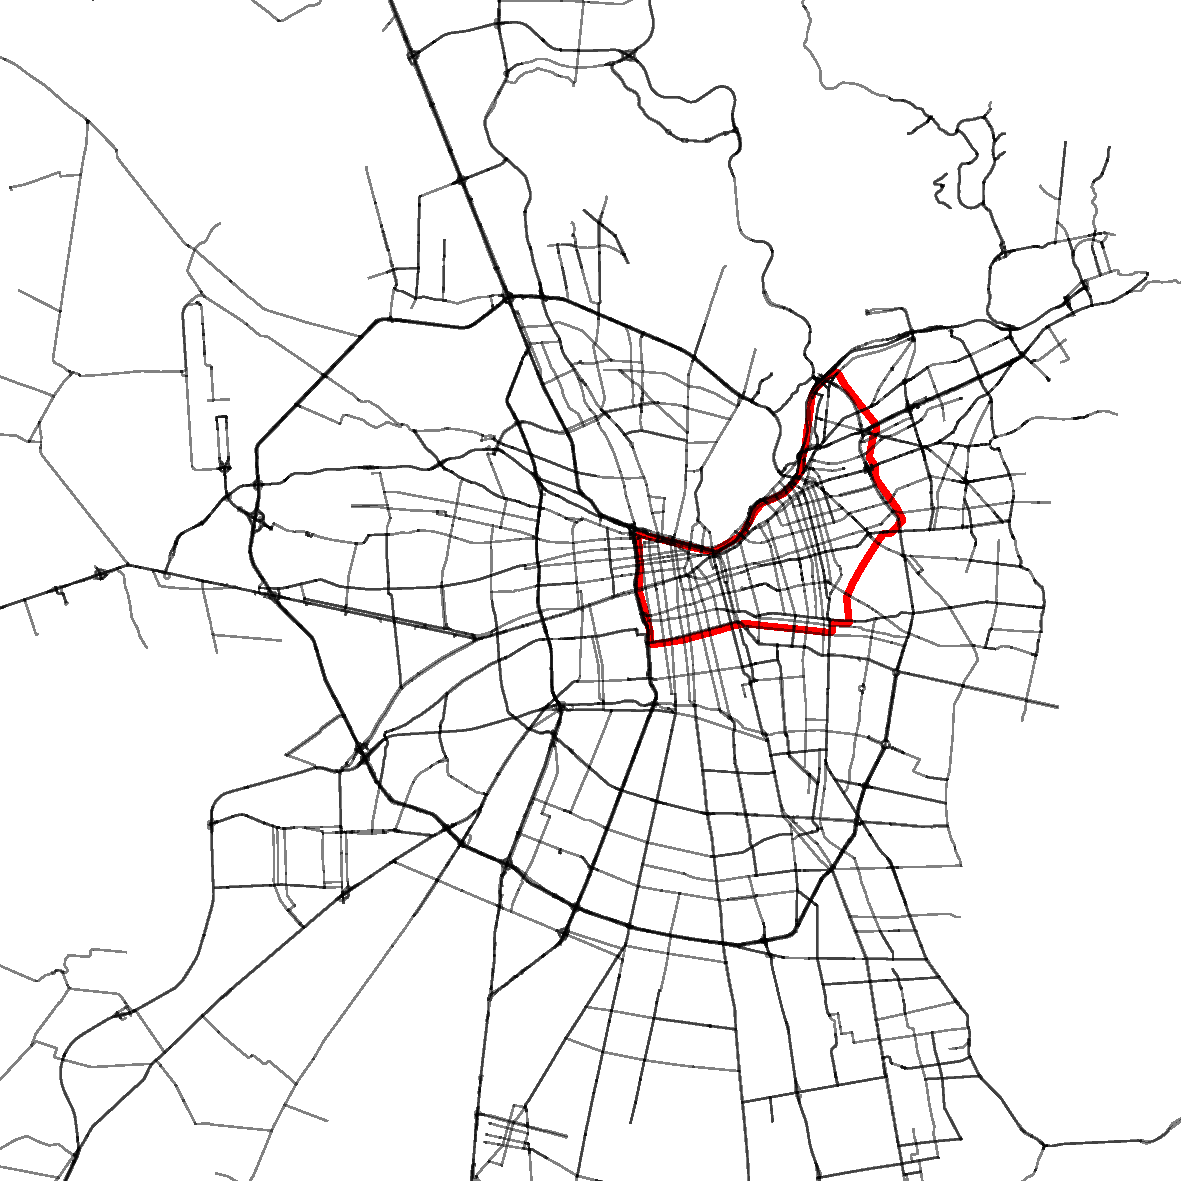
\includegraphics[scale=0.22]{images/outerCordon.pdf}\hspace{3cm}
	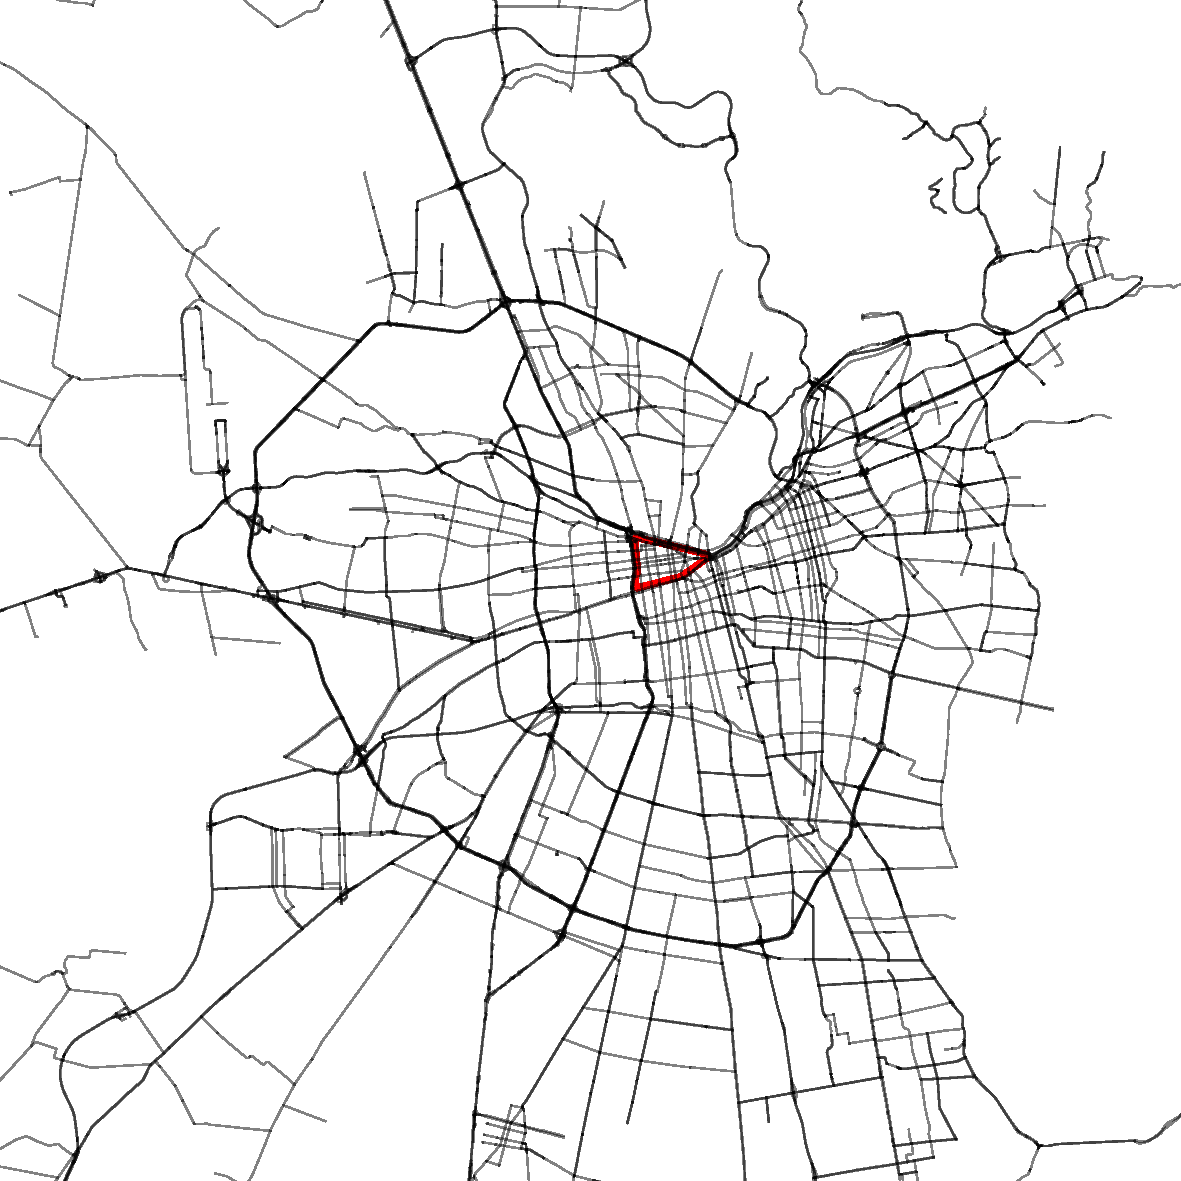
\includegraphics[scale=0.22]{images/triangleCordon.pdf}
	\caption{Cordon pricing schemes considered. Left: Outer Cordon. Right: Triangle Cordon}
	\label{fig:congestion_pricing_schemes}
\end{figure}

\begin{table}[h!]
	\centering
	\caption{Entry and exit charges in Outer and Triangle schemes. Source: \cite{gleave2009tarificacion}}
	\label{table:cordon_charges}
	\begin{tabular}{ccc}
		\hline
		Link type& Outer cordon charge {[}\$2001{]} & Triangle cordon charge{[}\$2001{]}\\
		\hline
		Entry & 6.000 & 6.000   \\
		Exit  & 3.600 & 2.650 \\
		\hline          
	\end{tabular}
\end{table}

\subsubsection{Results}

Daily modal splits variations for both 1\% and 10\% cases are shown in Figure \ref{fig:modal_split_results}. The results show a decrease in the modal split for car, and an increase in the modal split for public transport and walk modes, for both the 1\% and 10\% cases in the Outer and Triangle cordon scenarios (from now on, OT and TC, respectively), compared to the Stability Test with Innovation scenario (from now on ST). The magnitude of the variation in modal splits is clearly greater in the OC than in the TC scenario, in spite of the high fare magnitude considered. 

\begin{figure}[h!]
	\centering
	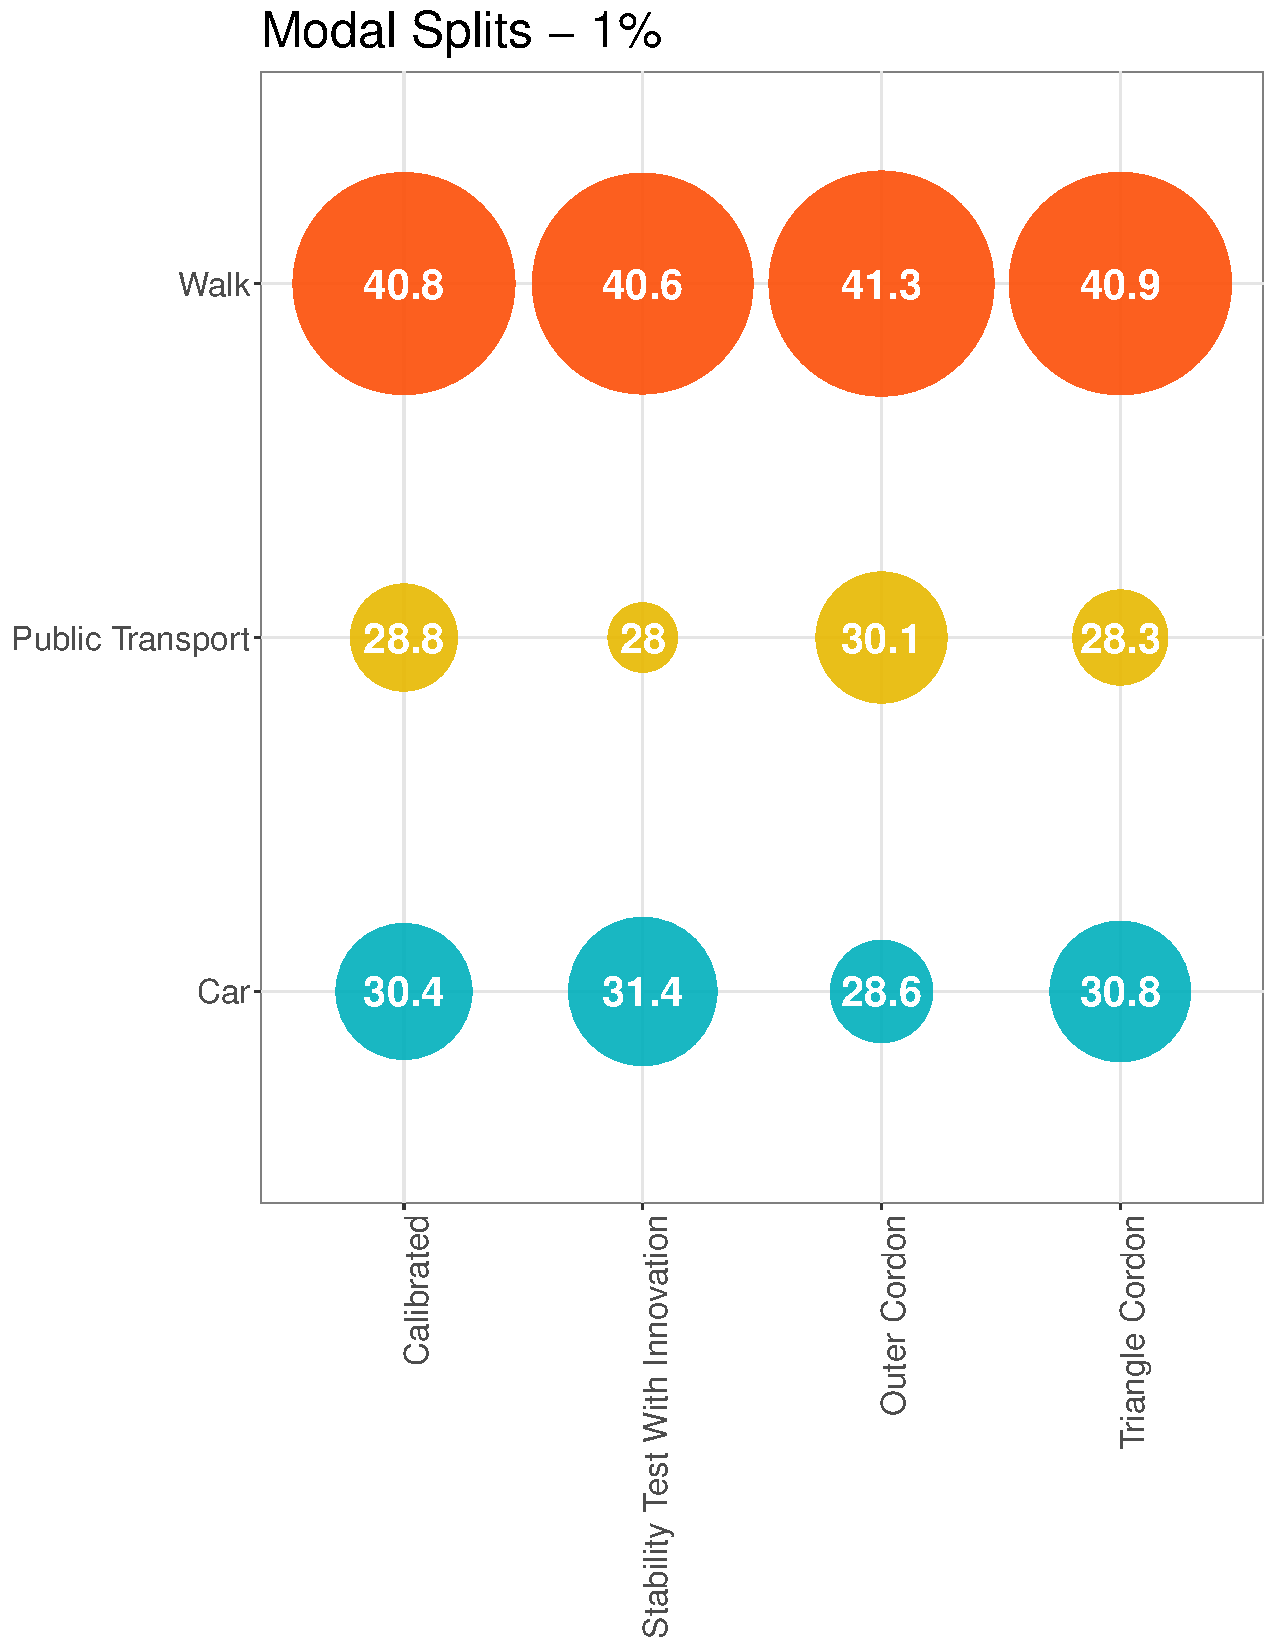
\includegraphics[scale=0.38]{images/modal_split_1pct.pdf}\hspace{0cm}
	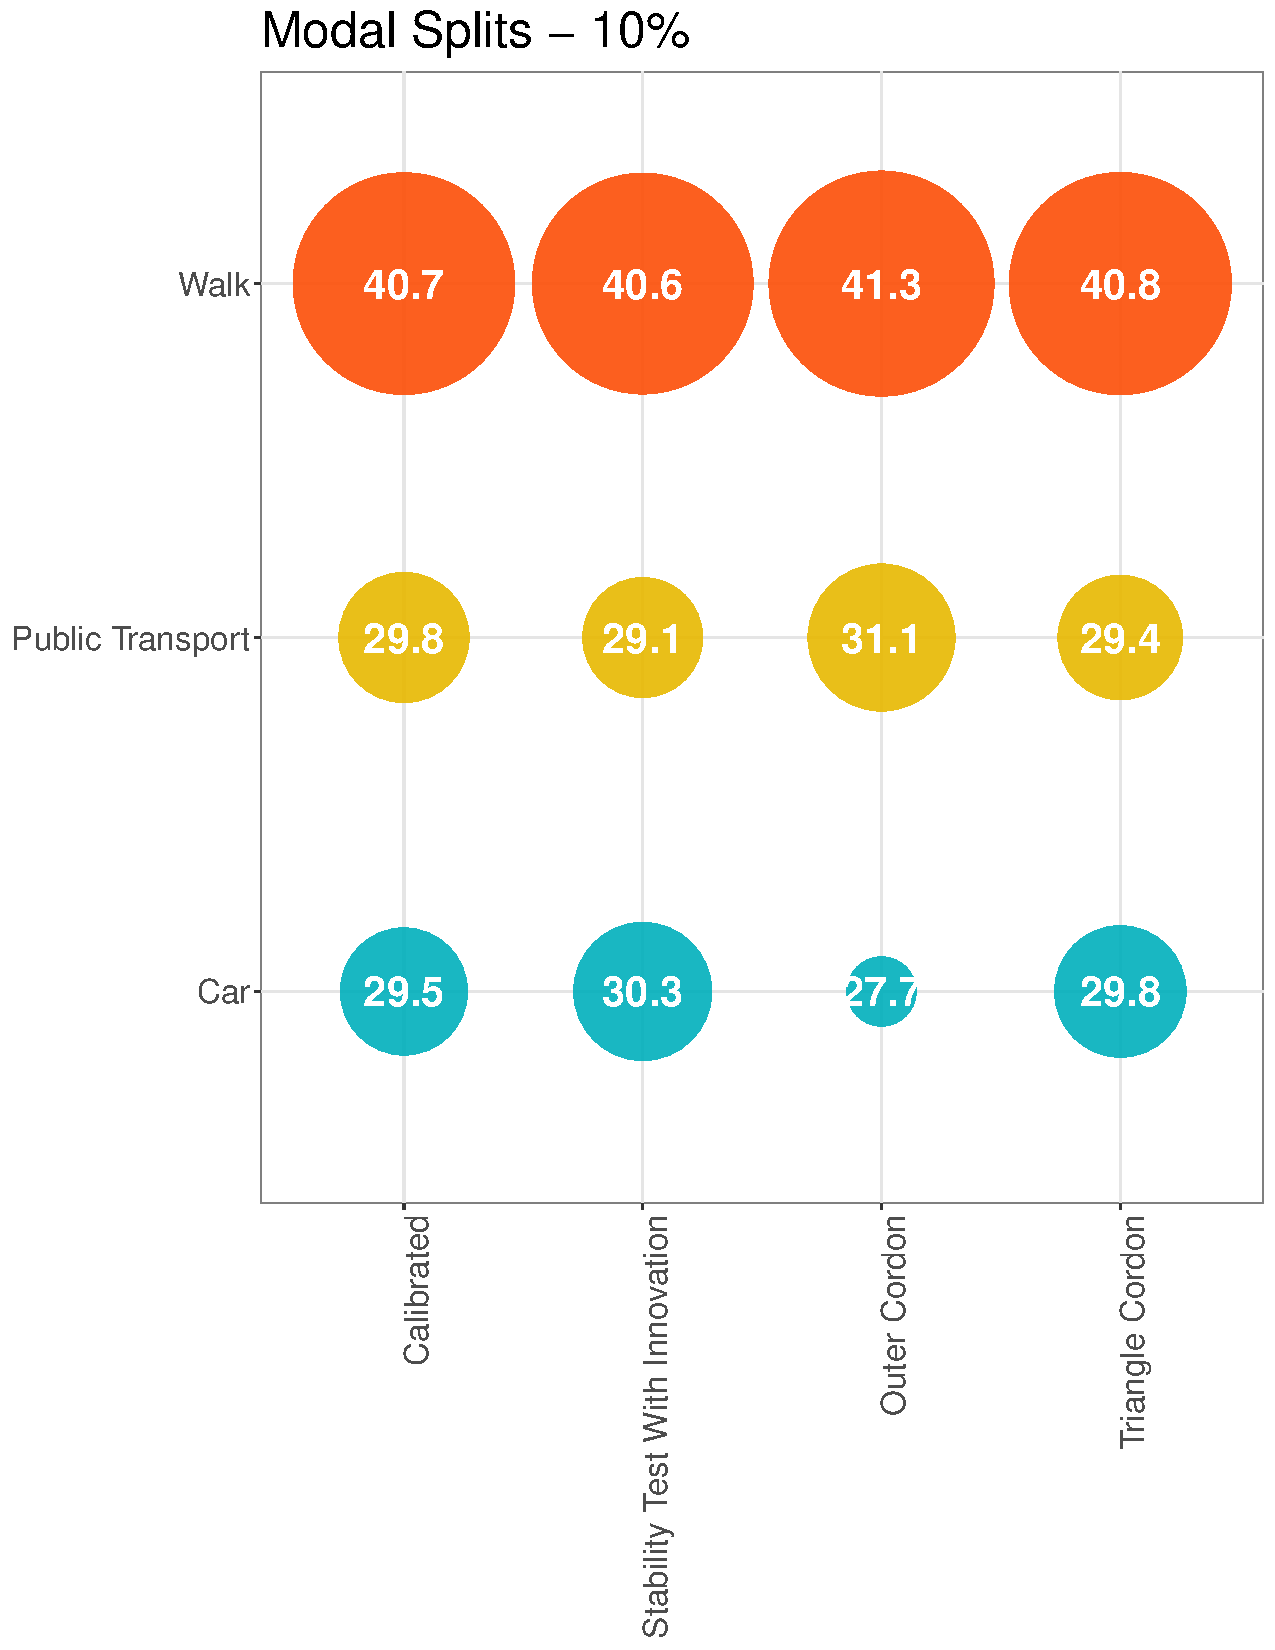
\includegraphics[scale=0.38]{images/modal_split_10pct.pdf}
	\caption{Modal splits variation. Left: 1\% case scenarios. Right: 10\% case scenarios}
	\label{fig:modal_split_results}
\end{figure}

The number of car legs for both 1\% and 10\% cases between 07:30 and 08:30 are summarized in Table \ref{table:legs_variation}, where OC-ST and TC-ST columns show the percentage change between the Outer Cordon and the Stability-Test scenario, and between Triangle Cordon and the Stability-Test scenario. These columns are useful to make a comparison with the results obtained by \cite{gleave2009tarificacion} for the same congestion schemes, where the percentage variations for car trips were found to be approximately -5\% and -1,5\% for the OC and the TC, respectively, compared to the base case. This reveals the agents greater sensibility to congestion pricing compared to the traditional modeling approach.

\begin{table}[h!]
	\centering
	\caption{Total car legs between 07:30 and 08:30.}
	\label{table:legs_variation}
	\begin{tabular}{ccc|cc|cc}
		\hline
		Case	& Calibrated & Stability-Test & Outer Cordon & OC-ST [\%] & Triangle Cordon & TC-ST [\%] \\
		\hline
		 1\%  & 3.028  & 3.176  & 2.431  & -23,46 & 3.035  & -4,44\% \\
		 10\% & 30.391 & 31.293 & 24.195 & -22,68 & 30.011 & -4,10\% \\
		\hline          
	\end{tabular}
\end{table}
%% Total travel time
Another interesting variable to analyze is the total traveled time and total traveled distances during 07:30 and 08:30, summarized in Table \ref{table:travel_time_variation} and Table \ref{table:travel_distance_variation}, respectively.

\begin{table}[h!]
	\centering
	\caption{Total traveled time consumed [hrs] between 07:30 and 08:30 by mode and case.}
	\label{table:travel_time_variation}
	\begin{tabular}{c|ccc|ccc}
		\cline{1-7}
				    & \multicolumn{3}{c|}{1\% case} & \multicolumn{3}{c}{10\% case} \\
		Scenario	& car    & pt    & walk  & car     & pt    & walk   \\ 
		\cline{1-7}
		Calibrated	& 1.259,49 	& 3.955,84	& 2.592,29	& 7.286,88	& 42.041,63 & 25.599,89  \\
		ST		 	& 1.547,63 	& 3.845,67	& 2.594,60	& 10.219,55	& 41.065,03 & 25.688,28  \\
		OC		 	& 989,24 	& 4.172,21 	& 2.714,39	& 6.642,63	& 44.203,02 & 26.631,29  \\
		TC		 	& 1.422,26 	& 3.897,62	& 2.627,95	& 9.698,05	& 41.552,48 & 25.911,17  \\
		\hline
		OC-ST [\%] 	& -36,08 & +8,49 & +4,62 & -35,00 & +7,64 & +3,67 \\		
		TC-ST [\%] 	& -8,10  & +1,35 & +1,29 & -5,10  & +1,19 & +0,87 \\					
		\cline{1-7} 
	\end{tabular}
\end{table}
%OK
Observing Table \ref{table:travel_time_variation}, it can be seen there exist a reduction in total traveled time in car mode and an increase in public transport and walk modes, for both congestion schemes and for 1\% and 10\% cases. Also, it can be seen that the 1\% case presents a higher variation in travel times for car mode compared to the 10\% case, result that should be seen with caution since the scenario scaling affects notoriously the travel time per kilometer distribution, as was already commented in Section \ref{sect:scaling_effect}. Table \ref{table:travel_time_variation_car_pt} shows the total traveled time percentage variation if only car and public transport mode are considered, results that can be compared with the results obtained by \cite{gleave2009tarificacion}. In this case, the travel time savings for the Outer Cordon in 1\% case are about three times higher than the saving for the Triangle Cordon scenario, results that are closer to the ones obtained in \cite{gleave2009tarificacion} who obtained savings for the Outer Cordon about two times higher compared to the Triangle Cordon. On the other hand, the Outer Cordon in 10\% case present travel time savings about twelve times higher than the ones for the Triangle Cordon scenario. 

\begin{table}
	\centering
	\caption{Percentage of variation in total traveled time consumed between 07:30 and 08:30 considering only car and public transport mode.}
	\label{table:travel_time_variation_car_pt}
	\begin{tabular}{ccc}
		\hline
		Scenario & 1\% case - $\Delta \mathit{t}$ [\%] & 10\% case - $\Delta \mathit{t}$ [\%] \\ 
		\hline
		OC-ST 	 & -4.30  & -0.86  \\
		TC-ST 	 & -1.36  & -0.07  \\ 
		\hline
	\end{tabular}
\end{table}

\begin{table}[h!]
	\centering
	\caption{Total traveled distance consumed [km] between 07:30 and 08:30 for car mode and for each case.}
	\label{table:travel_distance_variation}
	\begin{tabular}{c|cc}
		\cline{1-3}
		Scenario	& 1\% case - car  & 10\% case - car   \\ 
		\cline{1-3}
		Calibrated	& 25.200,25	& 239.364,48  \\
		ST			& 25.854,74	& 243.742,95  \\
		OC			& 20.478,37	& 194.222,39  \\
		TC			& 24.846,90	& 235.175,73  \\
		\hline
		OC-ST [\%] 	& -20,79 & -20,32 \\		
		TC-ST [\%] 	& -3,90  & -3,51  \\					
		\cline{1-3} 
	\end{tabular}
\end{table}

Finally, the total traveled distances summarized in Table \ref{table:travel_distance_variation} show little difference in the percentage variation between 1\% case and 10\% for same scenarios, result that is consistent with the one commented in Section \ref{sect:scaling_effect}. Again, it is found that the effect of the Outer Cordon is higher to the corresponding one in the Triangle Cordon, concluding the same as \cite{gleave2009tarificacion}. MATSim, however, estimates total travel distances percentage variations greater than the ones obtained in the previous study, which corresponds to $-5.8$\% and $-1.4$\% for the Outer Cordon and Triangle Cordon, respectively.

\section{Discussion and conclusions}

This work presented the development of an scenario and a first application of an agent-based model for the capital city of Chile. The MATSim model was used, which maintains the agents identity through the iterations, enabling to simulate the short and medium term decision processes such as route, mode or trip start time choices. In this model, agents move across the city in order to participate in different activities, which are capable to learn through the memorization of daily plans and their respective scores. 

First, a previous synthetic population \citep{MATSimSantiago} was enhanced in order to increase the resemble with the real Santiago's population: the number of agents was blown up using expansion factors determined by \cite{Contreras2015}, the activities location of the cloned agents were randomized using land-use data and their respective trip start times were modified using smartcard data, process that ended up with two scenarios representative of 1\% and 10\% of the total population of Santiago. In addition to this, some aspects of the network were improved, such as the addition of the tolls to the tollways. Later, the improved scenarios were calibrated in terms of modal splits calculated from the ODS and traffic counts from a previous study \citep{AFOROS2013}. Finally, both scenarios were used to asses a congestion pricing scheme and outputs (changes in daily modal splits, number of car legs, total traveled time by mode and total traveled distance in car mode) were compared to the ones obtained by \cite{gleave2009tarificacion}. In general, it was found that agents in MATSim reacted in a more sensitive way compared to ESTRAUS,  estimating a grater percentage of change in all the indicators analyzed in this study. 

Possible next steps of this work are continuing the scenario enhancement, this time in terms of public transport simulation using as input the GPS data of the public transport system of Santiago, together with a map matching algorithm. Also, it is highly necessary to explore other calibration methodologies, particularly automatic ones such as the Opdyts tool proposed by \cite{flotterod2017search}


\appendix
%
% And now for some pretty impressive notation.  In this example, I have used
%   the tabular environment to line up the columns in ASCE style.
%   Note that this and all appendices (except the references) start with 
%   the \section command
%

%\bibliographystyle{apalike-es}
\bibliography{ascexmpl-new}
% \label{section:references}

\end{document}
